%
% Chapter 7
%

\chapter{Background Estimation}
\label{bg_val}
% \epigraph{Nothing in life is to be feared, it is only to be understood. Now is the time to understand more, so that we may fear less.}{\textit{Marie Sklodowska Curie}}
% \vskip 0.5in

\section{Introduction}
The signal is a pair of oppositely charged leptons with different flavors, an isolated lepton, \Pe\, or \Pgm, accompanied by an isolated \Pgt (\taum, \taue, or \tauh) lepton. The dominant contribution for such a signature comes from \Ztt process, in which the \Pgm\, or \Pe\, arises from a \Pgt\, decay. The other dominant contribution comes from \wjets and QCD multijets processes, where one or more of the jets are misidentified as leptons. In the leptonic channels, the \ttbar process also has a dominant contribution.

Other contributions come from the processes in which a lepton pair is produced from the weak decays of quarks and vector bosons. These processes include Higgs boson production (\Htt, \PW{}\PW), \PW{}\PW, \PW{}\PZ, and \PZ{}\PZ. There are non-negligible contributions from processes like $\PW\Pgg^{(\ast)} +$ jets, single top quark production, and \Zll $(\ell=\Pe,\Pgm)$. Feynman diagrams of background processes to LFV Higgs boson decays are shown in Figure ~\ref{fig:feynman_bkg}.

The dominant contributors, \Ztt and misidentified lepton backgrounds, are estimated from data using either a fully data-driven or semi data-driven approach. All the other backgrounds are estimated from simulated samples. The background estimates are validated in different orthogonal control regions constructed to have enhanced contributions from the dominant backgrounds.

\begin{figure}[htbp!]
  \centering
  \subfigure[]{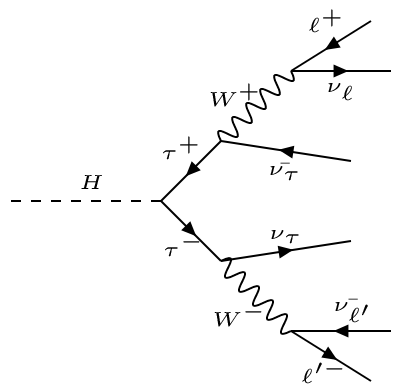
\includegraphics[width=0.3\textwidth]{plots/chapter7/Feynman/Htt.png}}
  \hspace{0.5cm}
  \subfigure[]{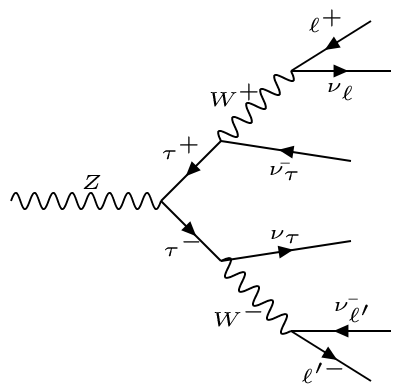
\includegraphics[width=0.3\textwidth]{plots/chapter7/Feynman/Ztt.png}}
  \hspace{0.5cm}
  \subfigure[]{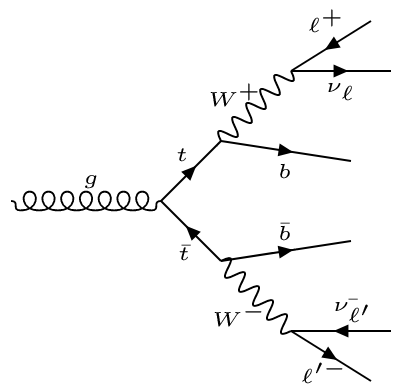
\includegraphics[width=0.3\textwidth]{plots/chapter7/Feynman/ttbar.png}}\\
  \vspace{1cm}
  \subfigure[]{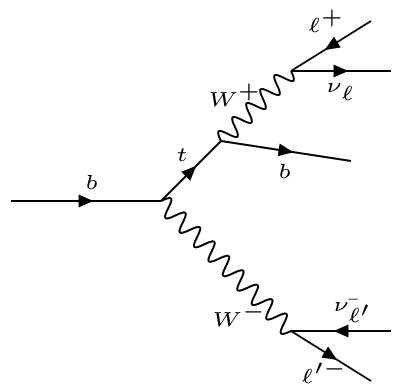
\includegraphics[width=0.3\textwidth]{plots/chapter7/Feynman/tW.png}}
  \hspace{0.5cm}
  \subfigure[]{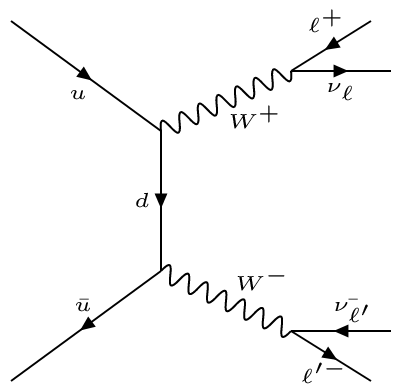
\includegraphics[width=0.3\textwidth]{plots/chapter7/Feynman/WW.png}}
  \hspace{0.5cm}
  \subfigure[]{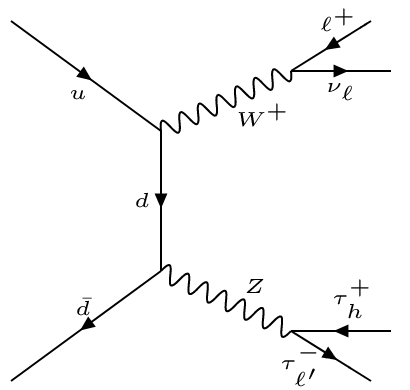
\includegraphics[width=0.3\textwidth]{plots/chapter7/Feynman/WZ.png}}\\
  \vspace{1cm}
  \subfigure[]{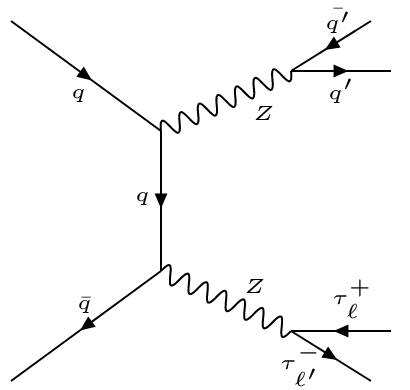
\includegraphics[width=0.3\textwidth]{plots/chapter7/Feynman/ZZ.png}}
  \hspace{0.5cm}
  \subfigure[]{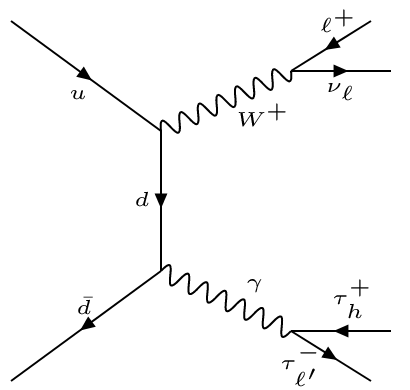
\includegraphics[width=0.3\textwidth]{plots/chapter7/Feynman/WG.png}}\\
  \caption{Feynman diagrams of background processes to LFV Higgs boson decays: (a) \Htt, (b) \Ztt, (c) \ttbar, (d) Single Top, (e) \PW{}\PW, (f) \PW{}\PZ, (g) \PZ{}\PZ, and (h) $\PW\Pgg^{(\ast)}$.}
  \label{fig:feynman_bkg}
\end{figure}

\section{Embedding technique}
The \Ztt background is estimated from data using the embedding technique ~\cite{Sirunyan:2019drn}. The embedding technique allows for an estimation of the genuine \Pgt{}\Pgt\, standard model backgrounds from data that minimizes uncertainties arising from a poor event description, with minimal simulation input. Events with a pair of oppositely charged muons are selected in data so that \Zmm events largely dominate it. These data events are chosen independently of the event selection criteria that are described in Chapter ~\ref{evt_sel}.

The muons are removed from the selected events and replaced with simulated \Pgt\, leptons with the same kinematic properties as that of the replaced muon. In that way, a set of hybrid events is obtained that relies on simulation only for the decay of the tau leptons. The description of the underlying event or the production of associated jets is taken entirely from data, and there is no reliance on the simulation. This technique results in a more accurate description of the \ptvecmiss, jet related variables, and an overall reduction in the systematic uncertainties that arise due to the usage of simulated samples.

Embedded samples cover all backgrounds with two real \Pgt\, leptons decaying semi-hadronically or leptonically. This includes a small fraction of \ttbar, Diboson, and electroweak \PW/\PZ\, events. The events from the \ttbar, Diboson, and electroweak \PW/\PZ\, MC samples where both tau candidates match genuine taus at the generator level are removed to avoid any double counting. A schematic for the embedding technique can be seen in Figure ~\ref{fig:embedding}.

\begin{figure}[htbp!]
  \centering
  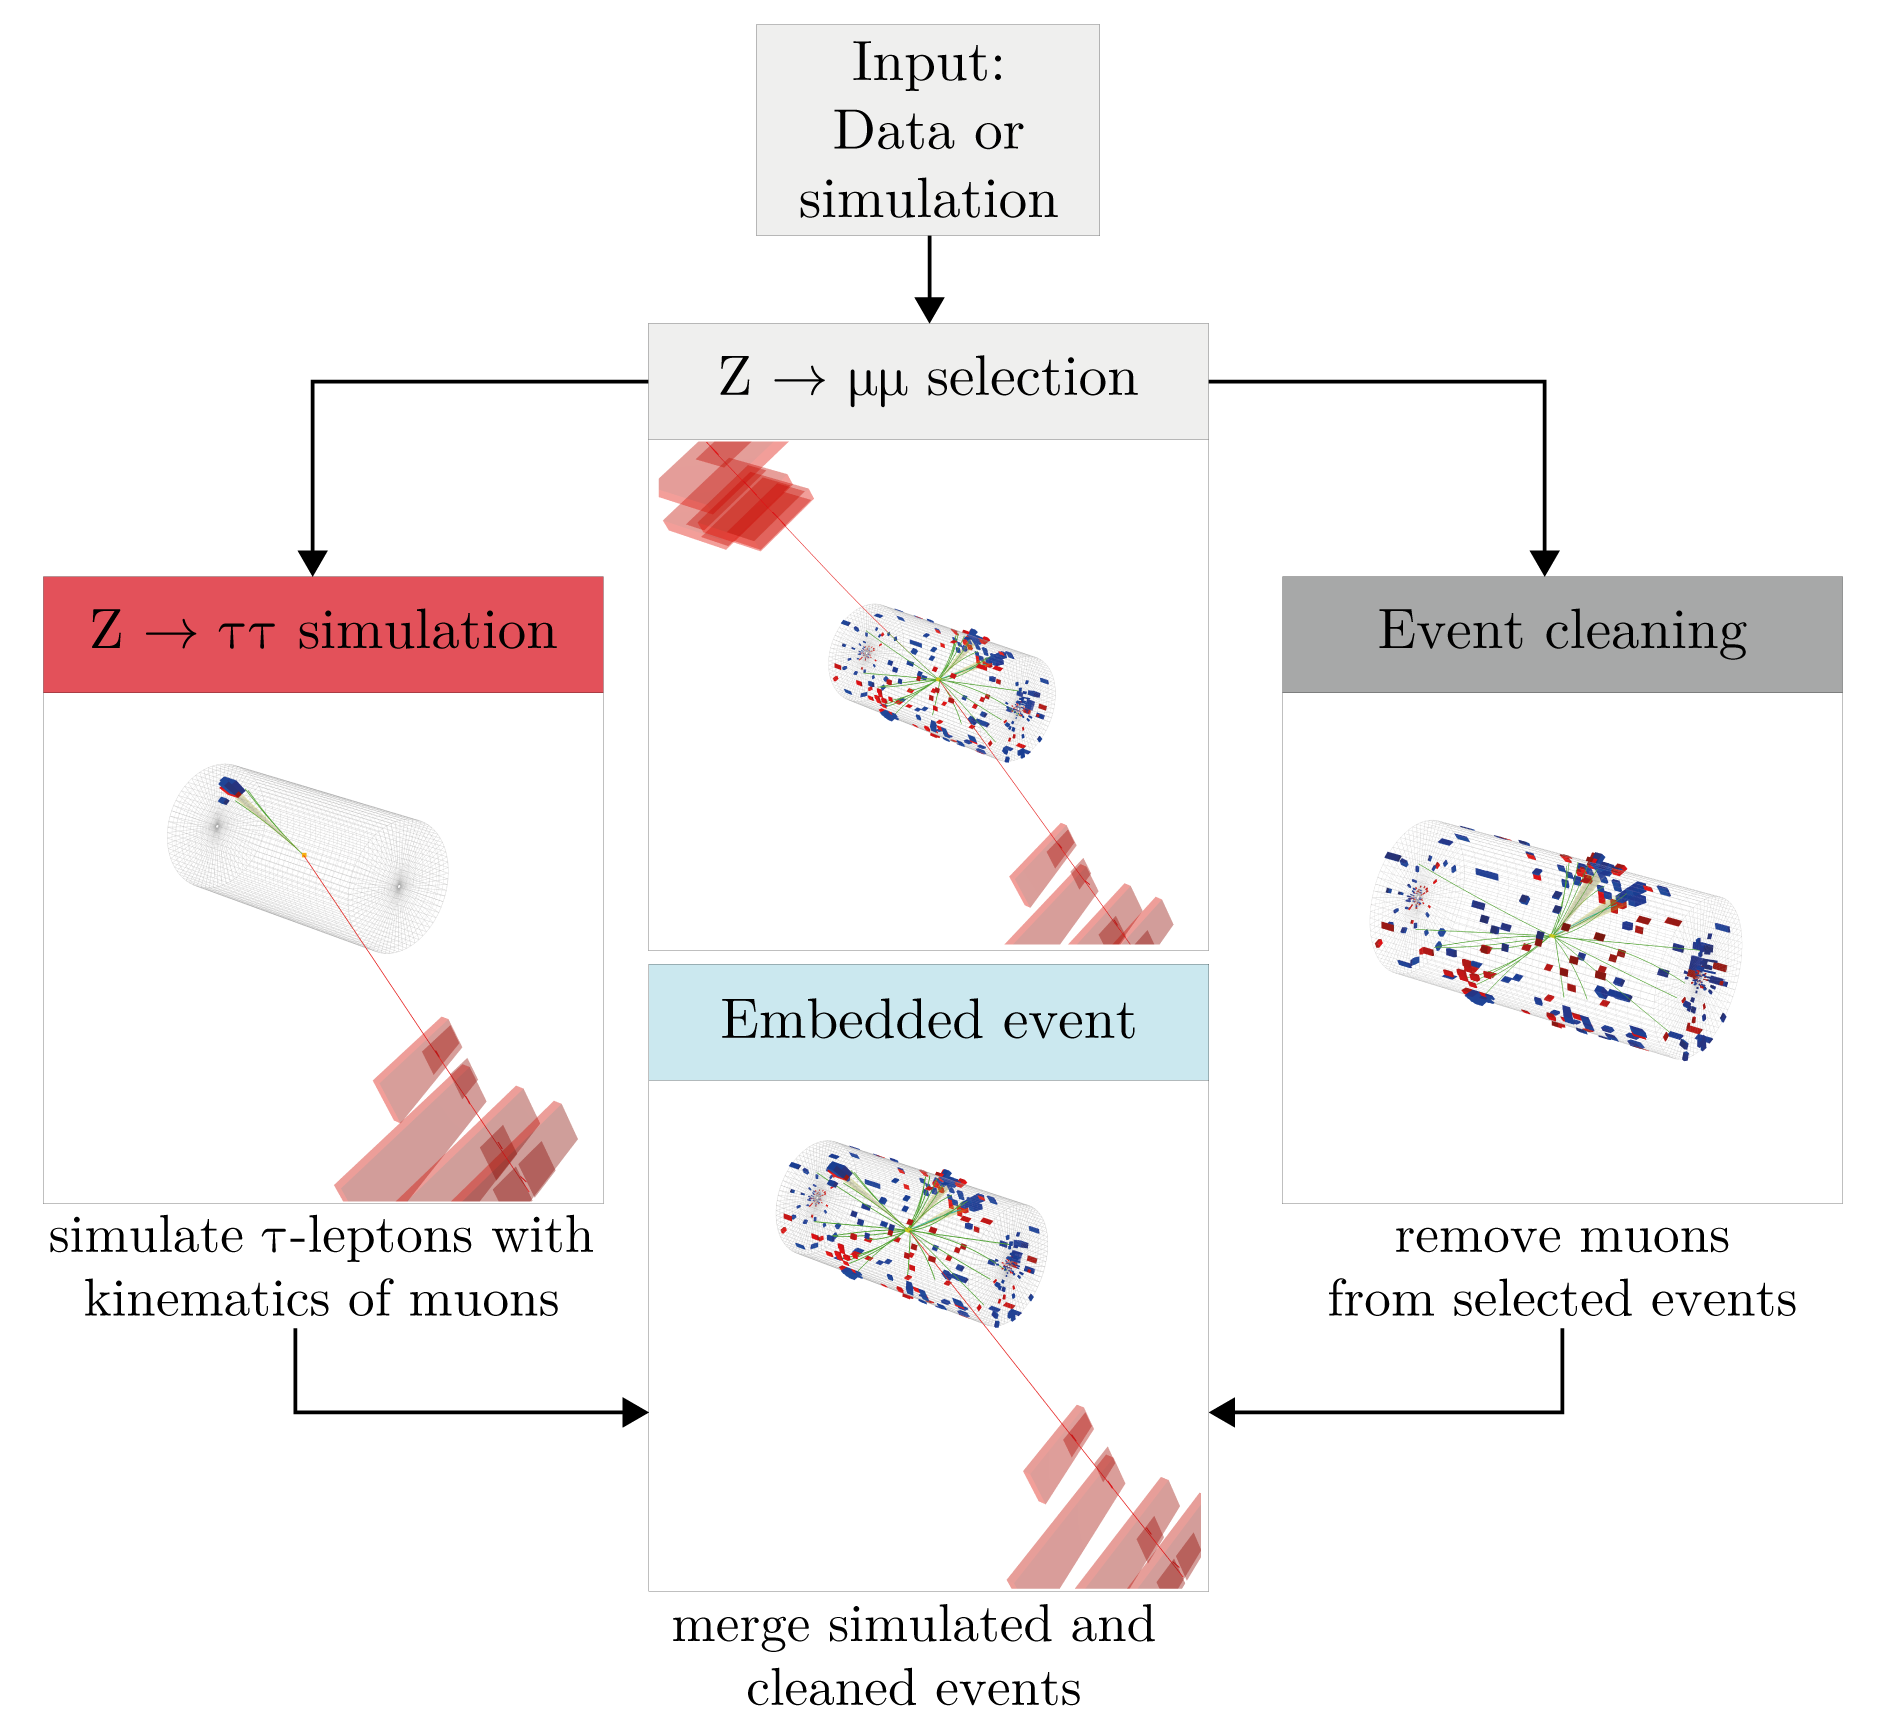
\includegraphics[width=0.8\textwidth]{plots/chapter7/emb.png}
  \caption{Schematic of Embedding Technique}
  \label{fig:embedding}
\end{figure}

The \Ztt background is validated by looking at the agreement between observed data and estimated background in a region enriched with \Ztt events. In \Hmuhad channel, this region is constructed by requiring, in addition to the preselection, $\mt(\Pgm) < 40\GeV$, $40\GeV < \mvis(\Pgm, \Pgt) < 80\GeV$, and $\pzeta(\Pgm, \Pgt) > -25$. \pzeta is the difference of the projections of $\pt^{\ell}$ plus MET, and the $\pt^{\ell}$ on the axis bisecting the two leptons. In \Hehad channel, the same requirements are placed with the muon variables replaced by corresponding electron variables.

In \Hmue channel, this region is constructed by requiring, in addition to the preselection, $\mt(\Pgm) < 60\GeV$, $30\GeV < \mvis(\Pgm, \Pe) < 70\GeV$, and $\pt^{\Pgm} < 40\GeV$. In \Hemu channel, the same requirements are placed with the muon variables replaced by corresponding electron variables and vice versa. Figures ~\ref{fig:ztt_control} and ~\ref{fig:ztt_control_BDT} show the comparison of data with background estimates in the \Ztt control regions for the \Hmt and \Het channels.

\begin{figure}[htbp!]
  \centering
  \subfigure[]{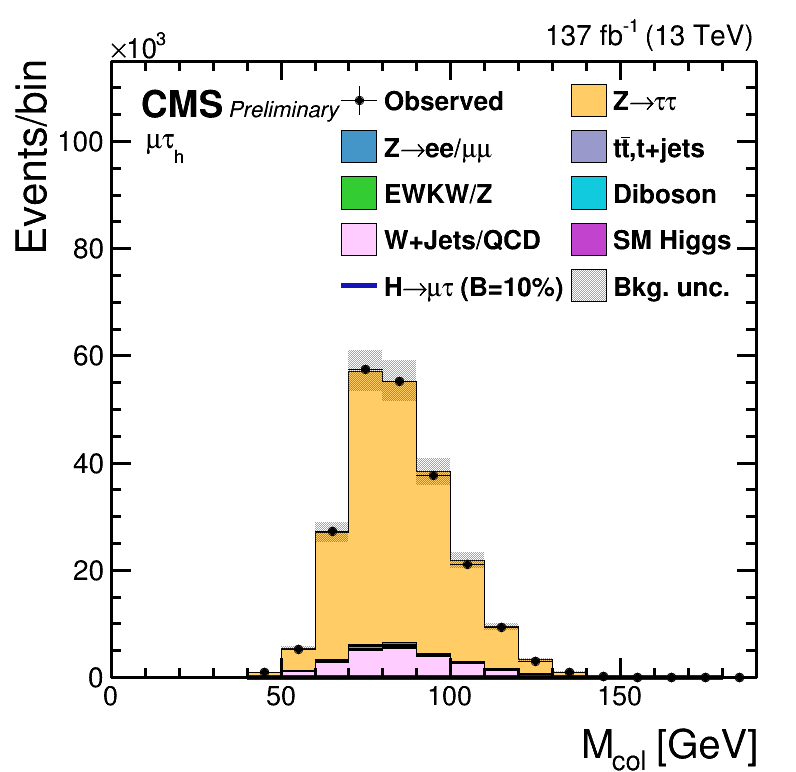
\includegraphics[width=0.45\textwidth]{plots/chapter7/Fake/mutau/ZTT.png}}
  \subfigure[]{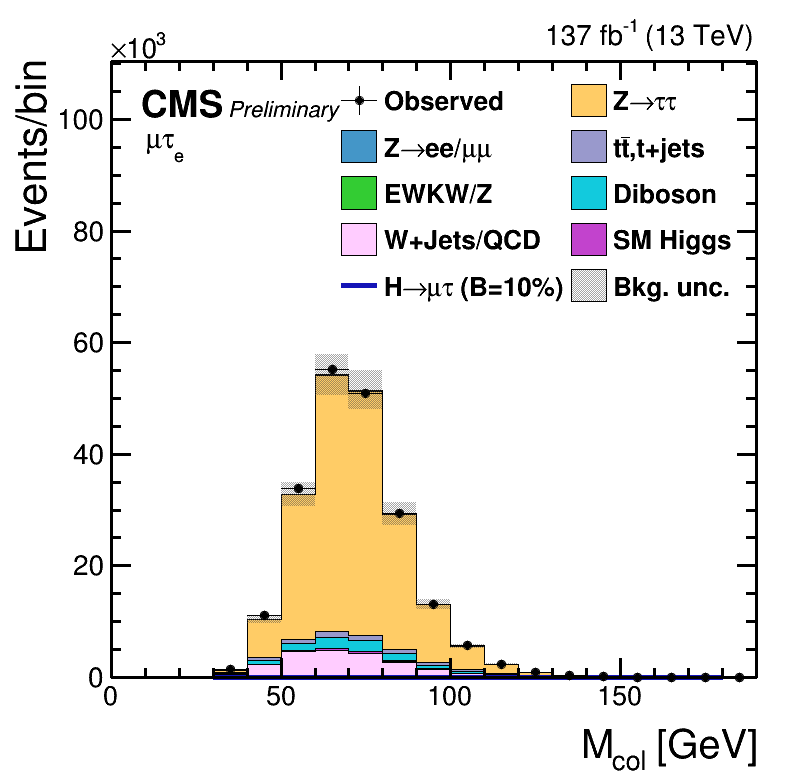
\includegraphics[width=0.45\textwidth]{plots/chapter7/Fake/mue/ZTT.png}}
  \subfigure[]{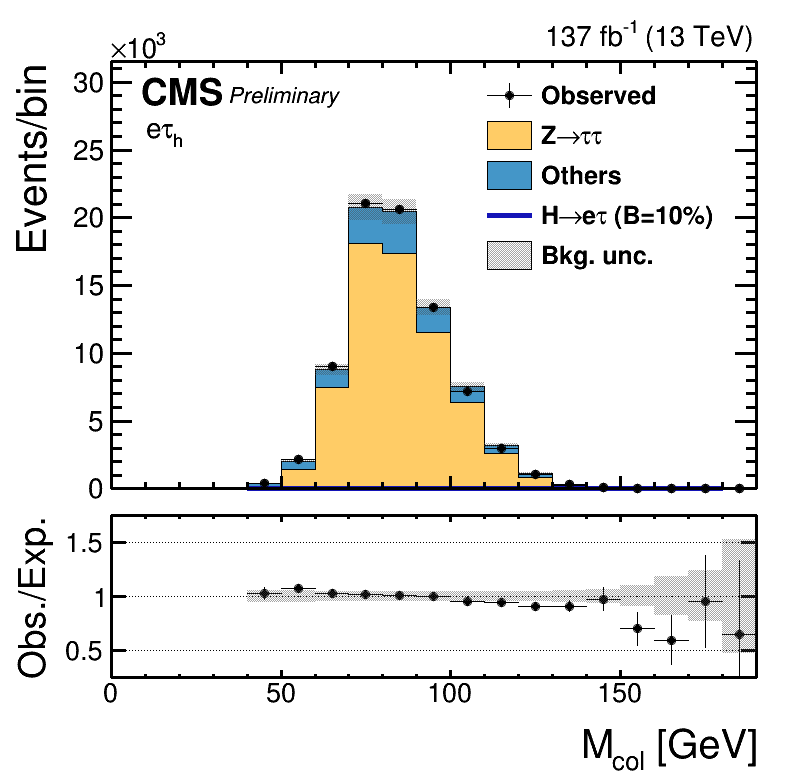
\includegraphics[width=0.45\textwidth]{plots/chapter7/Fake/etau/ZTT.png}}
  \subfigure[]{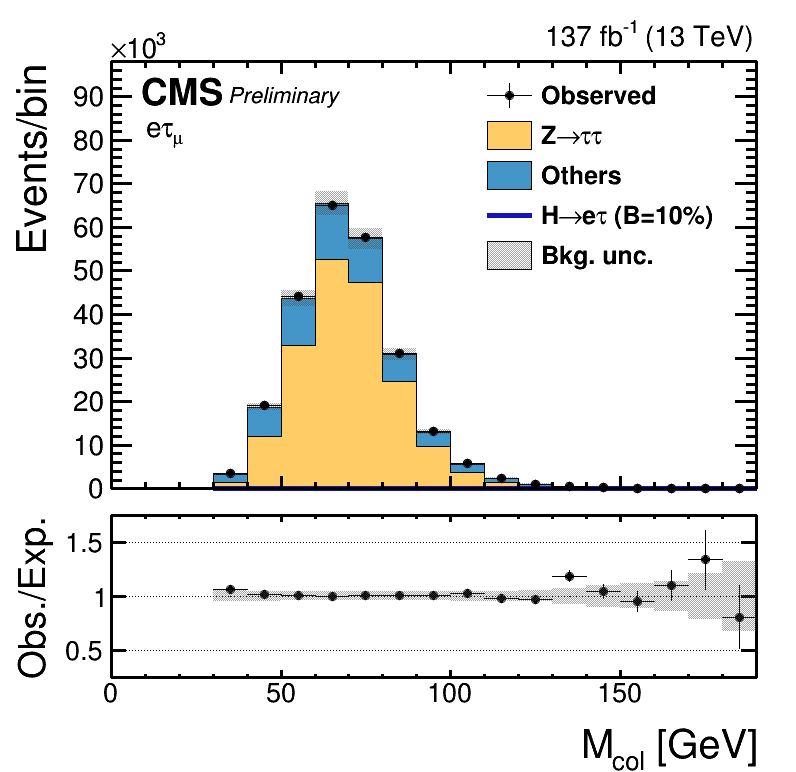
\includegraphics[width=0.45\textwidth]{plots/chapter7/Fake/emu/ZTT.png}}
  \caption{Distributions of \mcol discriminator in the \Ztt control regions for the (a) \Hmuhad, (b) \Hmue, (c) \Hehad, and (d) \Hemu channels.}
  \label{fig:ztt_control}
\end{figure}

\begin{figure}[htbp!]
  \centering
  \subfigure[]{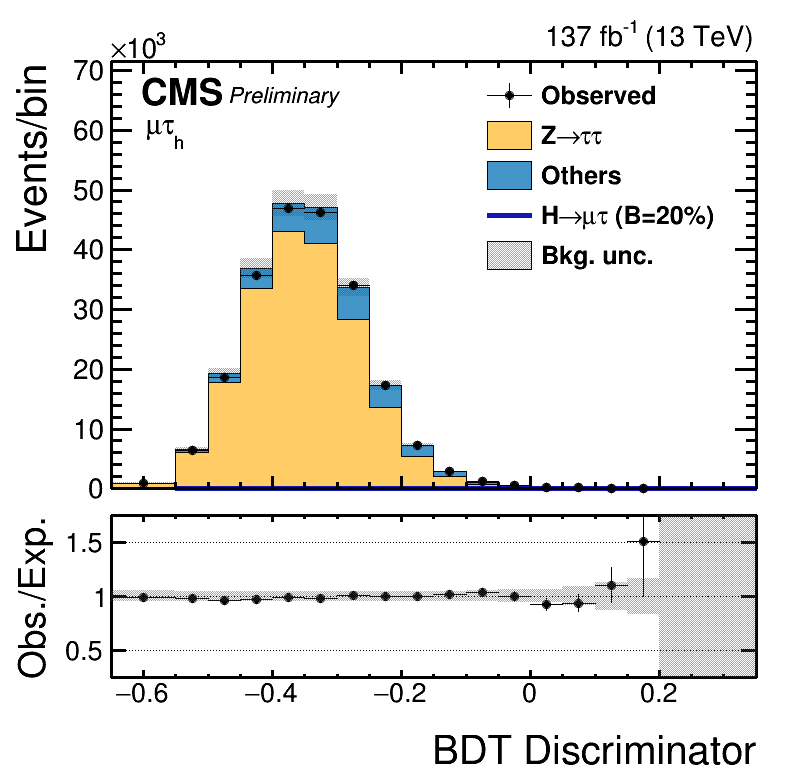
\includegraphics[width=0.45\textwidth]{plots/chapter7/Fake/mutau/ZTTBDT.png}}
  \subfigure[]{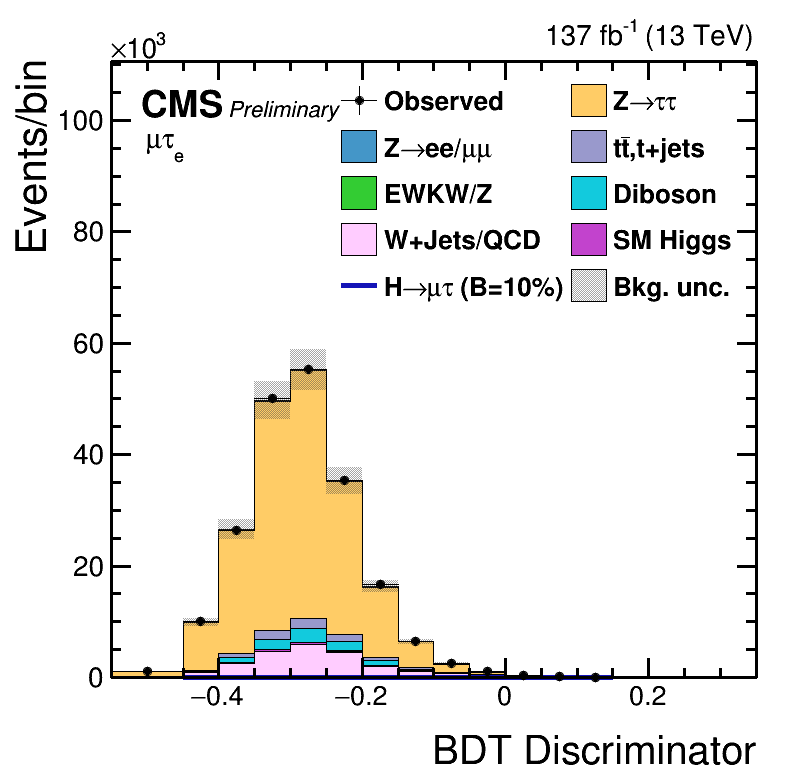
\includegraphics[width=0.45\textwidth]{plots/chapter7/Fake/mue/ZTTBDT.png}}
  \subfigure[]{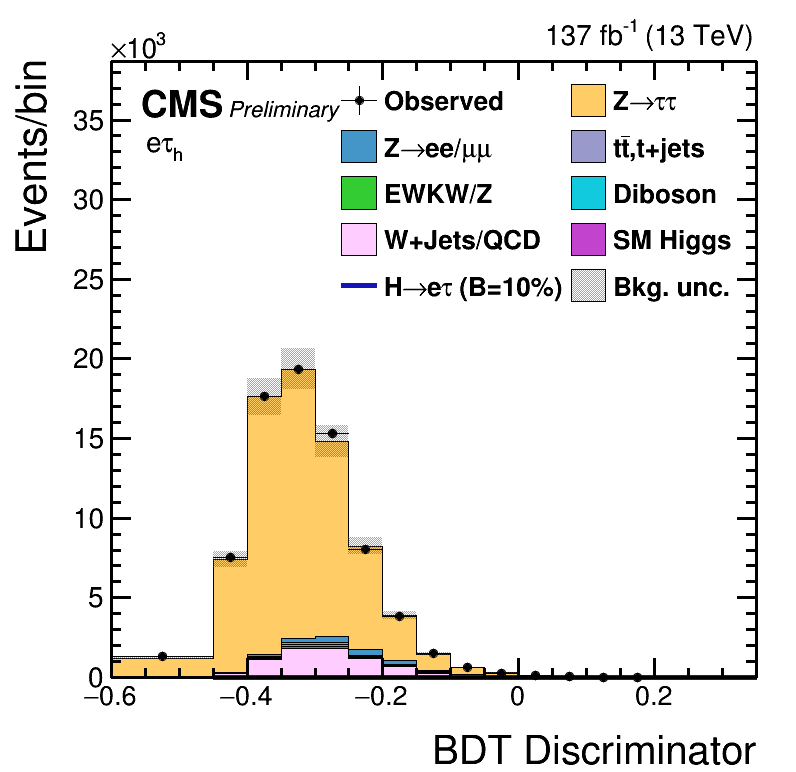
\includegraphics[width=0.45\textwidth]{plots/chapter7/Fake/etau/ZTTBDT.png}}
  \subfigure[]{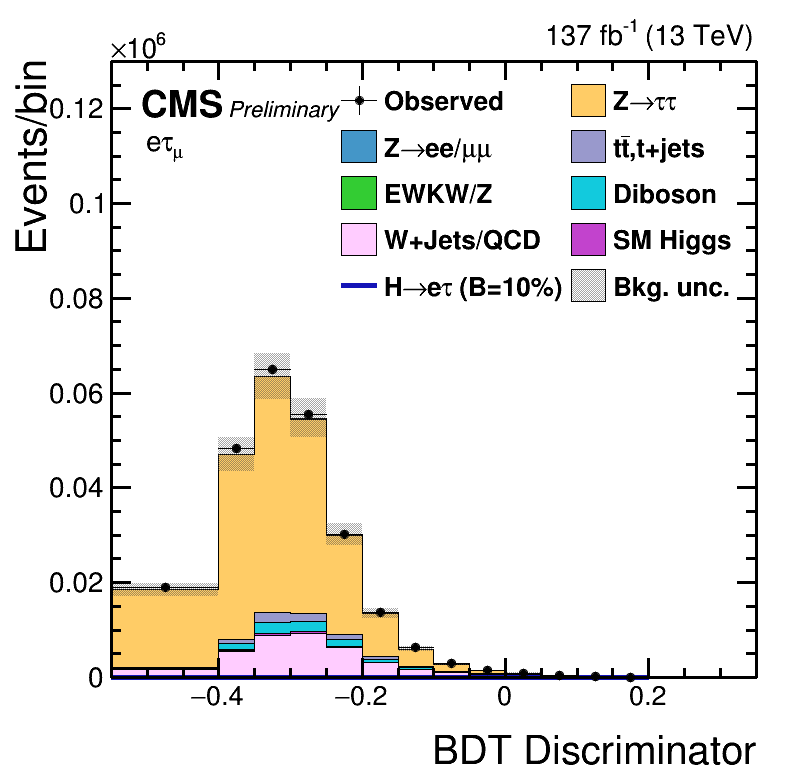
\includegraphics[width=0.45\textwidth]{plots/chapter7/Fake/emu/ZTTBDT.png}}
  \caption{Distributions of BDT discriminator in the \Ztt control regions for the (a) \Hmuhad, (b) \Hmue, (c) \Hehad, and (d) \Hemu channels.}
  \label{fig:ztt_control_BDT}
\end{figure}

\section{Misidentified lepton background}
Misidentified lepton background corresponds to processes where jets are misidentified as leptons. They mostly arise from two sources, \wjets, and QCD multijet events. In \wjets background events, one of the lepton candidates is from the \PW\, boson decay while the other is a jet misidentified as a lepton. In QCD multijet events, both the lepton candidates are misidentified jets.

In two channels of this analysis (\muhad and \ehad), the contributions from misidentified lepton backgrounds have been estimated using a fully data-driven approach. In the leptonic channels (\mue and \emu), a semi data-driven approach is adopted. The results from the semi-data driven approach are found consistent with the fully data-driven method and are undertaken due to limited statistics in the leptonic channel.

\subsection{Fully data-driven approach}
The misidentified lepton background is estimated from collision data by defining a control region with the same selection as the signal region, but loosening the isolation requirements on one of the leptons, to enrich the contribution from \wjets and QCD multijets. The misidentification rates are evaluated using events with a \PZ\, boson candidate, and at least one jet that can be misidentified as a lepton and then applied to the control region, to estimate the misidentified background of the signal region. The signal region contrasted with the control regions used for determining the misidentified background can be seen in Figure ~\ref{fig:fake}.

\begin{figure}[hbtp!]
  \centering
  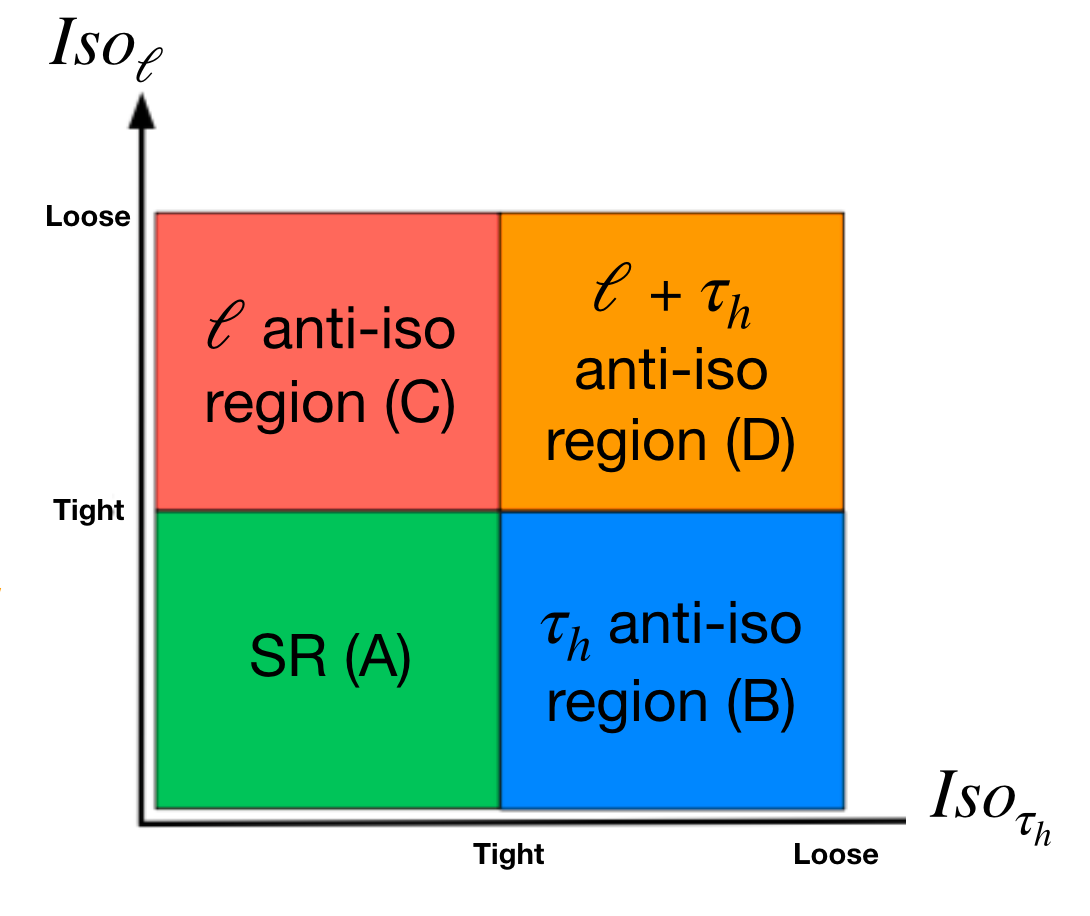
\includegraphics[width=0.49\textwidth]{plots/chapter7/Fake/Fake.png}
  \caption{Signal region (green) contrasted with the control regions used for estimating the misidentified background}
  \label{fig:fake}
\end{figure}

The probabilities with which jets are misidentified as an electron, muon, or hadronically decaying tau are labeled as $f_\Pe, f_\Pgm$, and $f_{\tauh}$, respectively. The \PZ\, boson candidate is formed using two muons with $\pt^\Pgm > 26\GeV$ and $\abs{\eta} < 2.4$ and $I^\ell_{\text{rel}} < 0.15$ for measuring the jet $\to\tauh, \Pgm, \Pe$ misidentification rate. The muons are required to be oppositely charged and have their invariant mass ($M_{\Pgm\Pgm}$) between 70 and $110\GeV$.

The contribution from diboson events, where the jet candidate corresponds to a real lepton, is subtracted using simulation. The jet is required to pass the same lepton identification criteria as used in the signal region. A ``signal-like'' sample is defined if the jet passes the tight lepton isolation, else a ``background-like'' sample is defined if it only passes the looser lepton isolation. These two samples are used to estimate $f_\Pe, f_\Pgm,$ and $f_{\tauh}$ using the following:
\begin{linenomath*}
  \begin{equation*}
    f_{i} = \frac{N_i(\text{signal-like})}{N_{i}(\text{background-like}) + N_i(\text{signal-like})}
  \end{equation*}
\end{linenomath*}
where $N_i(\text{signal-like})$ is the number of events with a third lepton candidate that passes the tight lepton isolation, while $N_i(\text{background-like})$ is the number of events that pass only the looser lepton isolation and index $i = \Pe, \Pgm,$ or \Pgt. The lepton selection criteria is summarized in Tables ~\ref{tab:mutau_evtselection} and ~\ref{tab:etau_evtselection}.

To estimate the misidentified \Pgm\, and \Pe\, contribution in the background-like category, lepton isolation is required to be $0.15 < I^\Pgm_{\text{rel}} < 0.25$ and $0.15 < I^\Pe_{\text{rel}} < 0.5$, respectively. The misidentification rate is computed as a function of the lepton \pt. To estimate the \tauh misidentified contribution, \tauh candidates are required to pass the loose Working Point (WP) of Deep Neural Network (DNN) discrimination against jets but fail the tight WP used for the signal selection. The \tauh misidentification rate shows a \pt\, dependence that varies with the \Pgt\, decay mode and $\abs{\eta}$ and are thus evaluated as a function of $\pt^{\Pgt}$ for the different decay modes and two $\abs{\eta}$ regions ($\abs{\eta} < 1.5$ or $\abs{\eta} > 1.5$).

In the \Hehad channel, the \tauh misidentification rate is evaluated using events with a \PZ\, boson candidate that is formed using two electrons with $\pt^\Pe > 27\GeV$ and $\abs{\eta} < 2.5$ and $I^\ell_{\text{rel}} < 0.15$. The electrons are required to be oppositely charged and have their invariant mass ($M_{\Pe\Pe}$) between 70 and $110\GeV$. The reason for using \Zee events for evaluating the \tauh misidentification rate in \Hehad channel is because the DNN WPs used for discriminating \tauh against electrons and muons is different in this channel compared to the \Hmuhad channel. The misidentification rates that are evaluated using this control region are compatible with the measurement in \Zmm events.

\begin{figure}[htbp]
  \centering
  \subfigure[]{
    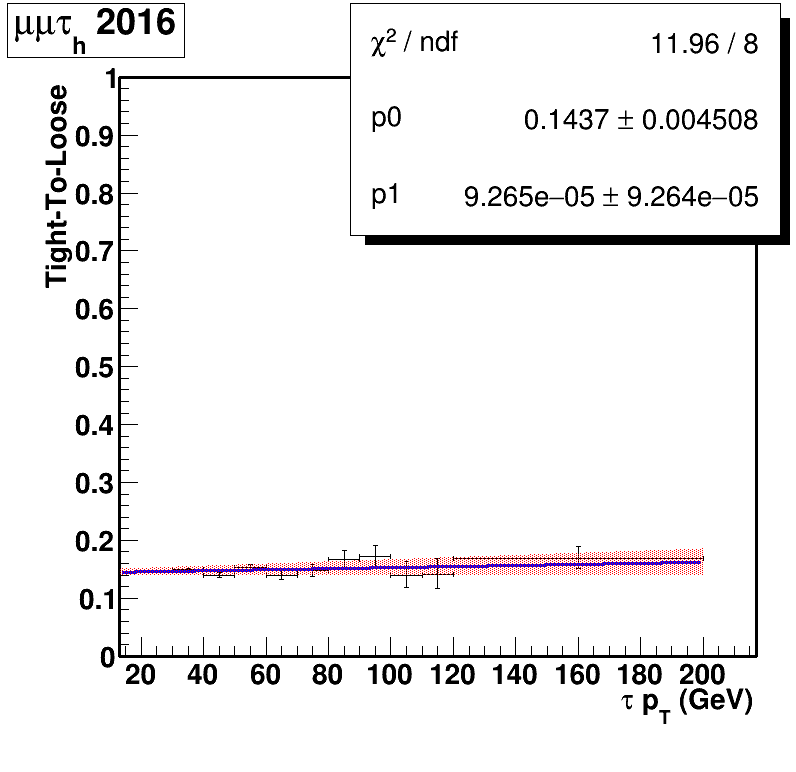
\includegraphics[width=0.3\textwidth]{plots/chapter7/Fake/FR/MMT2016.png}
    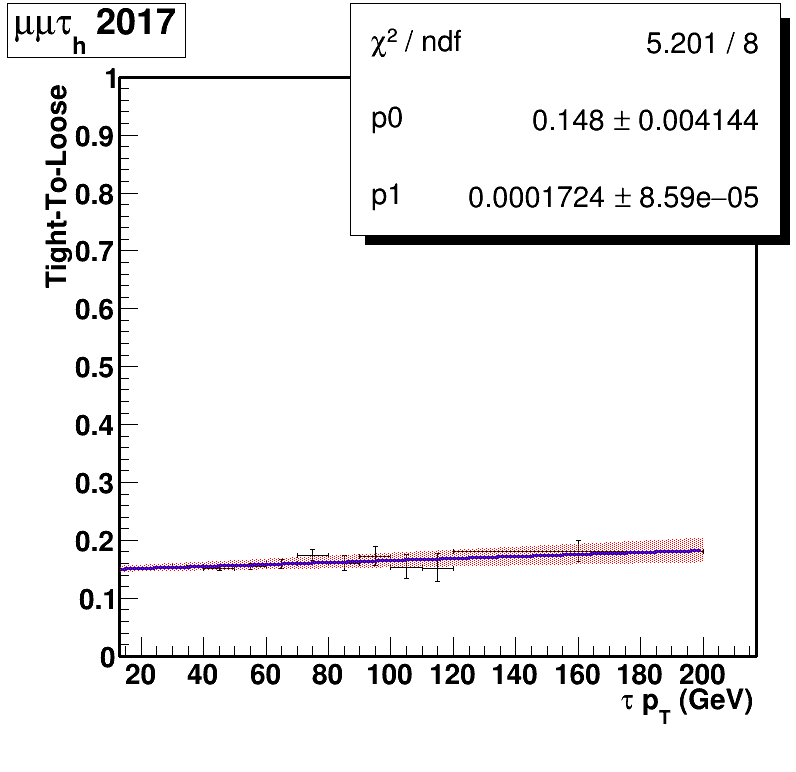
\includegraphics[width=0.3\textwidth]{plots/chapter7/Fake/FR/MMT2017.png}
    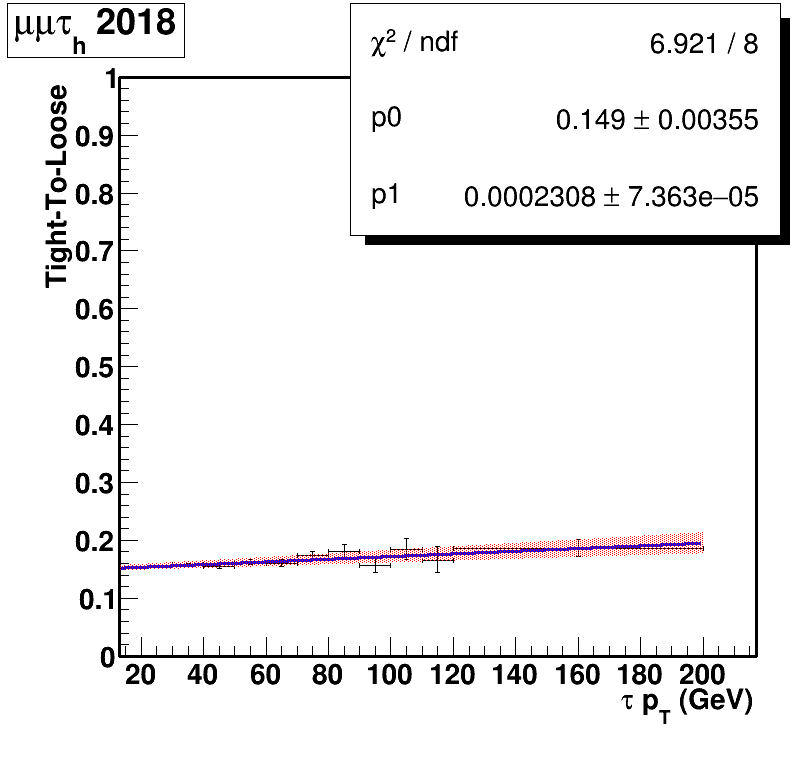
\includegraphics[width=0.3\textwidth]{plots/chapter7/Fake/FR/MMT2018.png}
  }
  \subfigure[]{
    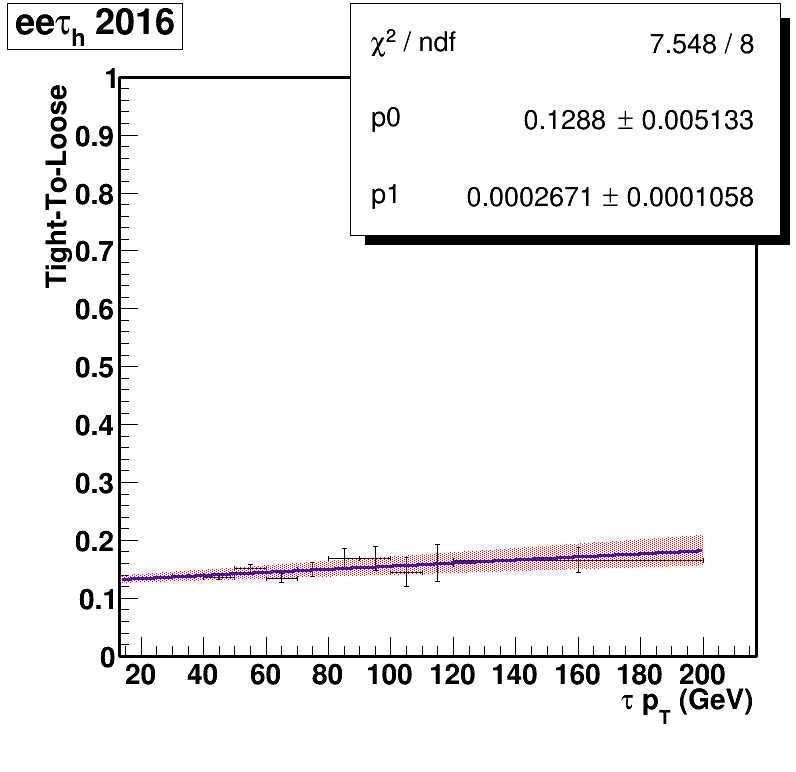
\includegraphics[width=0.3\textwidth]{plots/chapter7/Fake/FR/EET2016.png}
    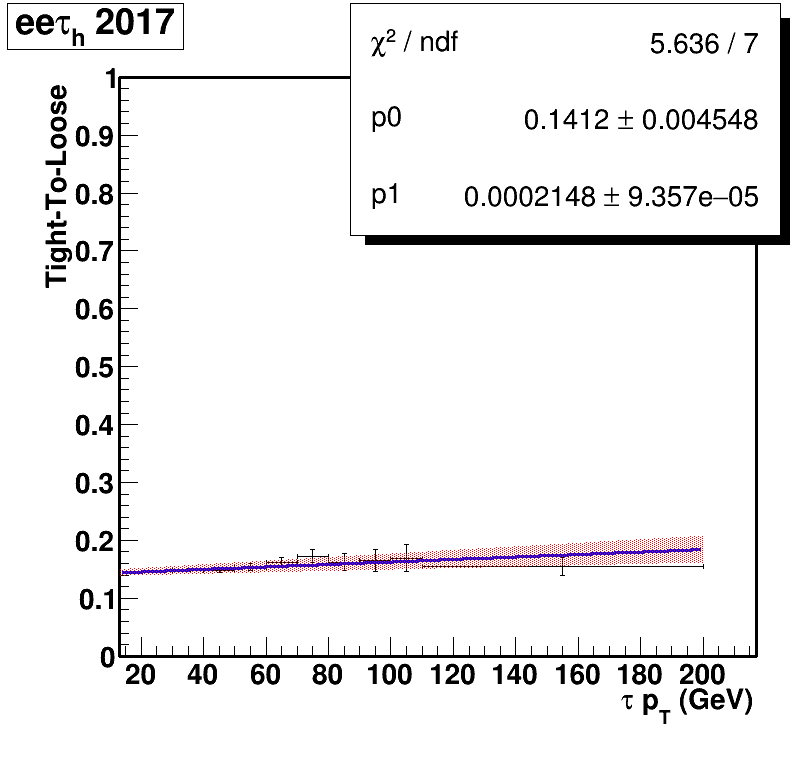
\includegraphics[width=0.3\textwidth]{plots/chapter7/Fake/FR/EET2017.png}
    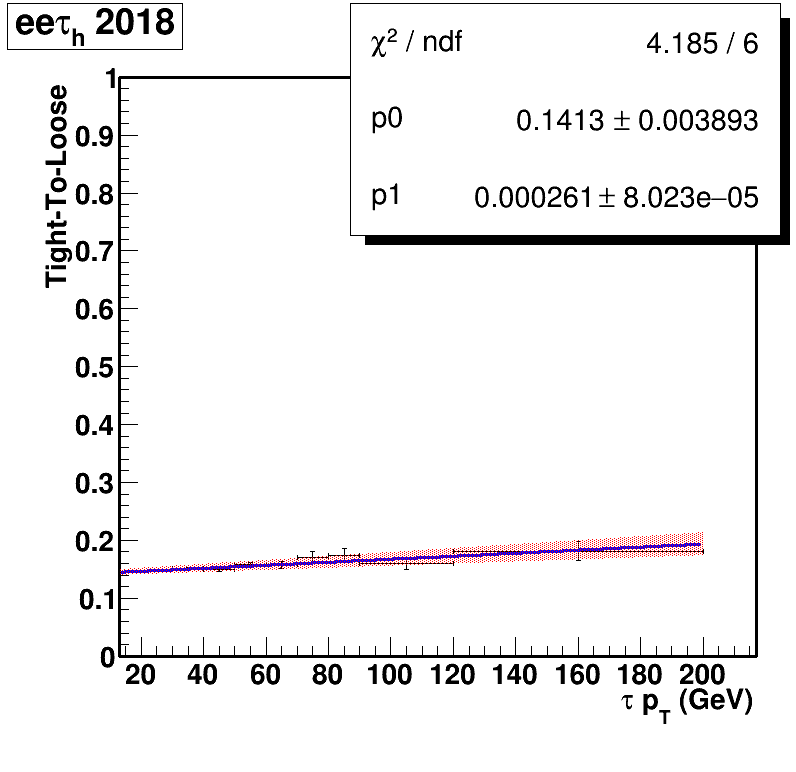
\includegraphics[width=0.3\textwidth]{plots/chapter7/Fake/FR/EET2018.png}
  }
  \caption{Fit performed to \tauh misidentification rates for \Hmuhad (a) and \Hehad (b) channel as a function of \tauh \pt\, for the different years. The misidentification rates used are further parametrized based on \tauh Decay Mode along with the pseudorapidity of \tauh. However, here only the inclusive misidentification rates are shown. The misidentification rates are labeled as ``tight-to-loose'' to clarify that they are calculated as a ratio of the number of events passing the tight WP to the loose WP of DNN discrimination against jets.}
  \label{fig:fakerate_tauh}
\end{figure}

\begin{figure}[htbp]
  \centering
  \subfigure[]{
    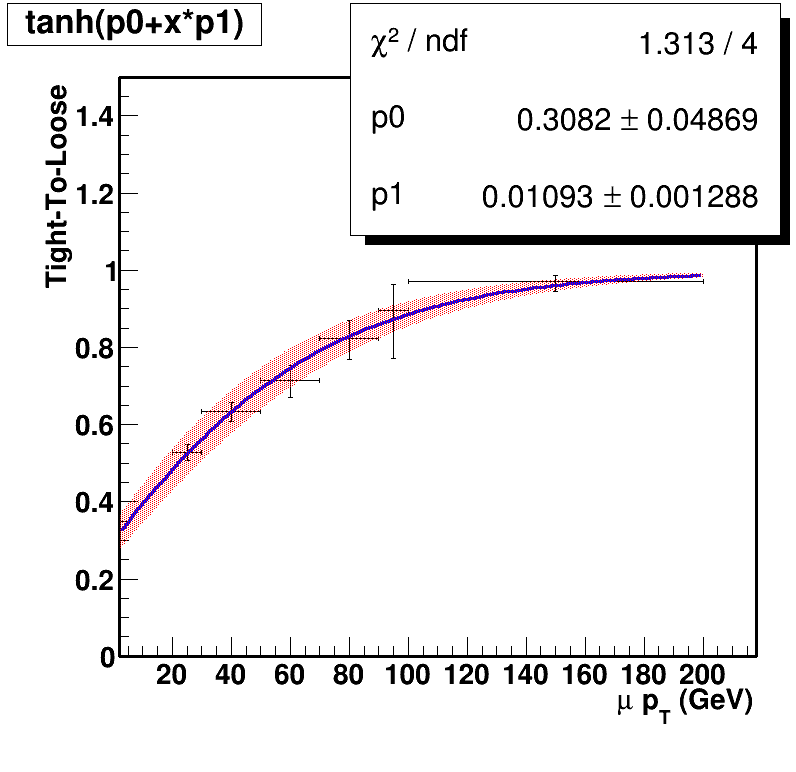
\includegraphics[width=0.3\textwidth]{plots/chapter7/Fake/FR/MMM2016.png}
    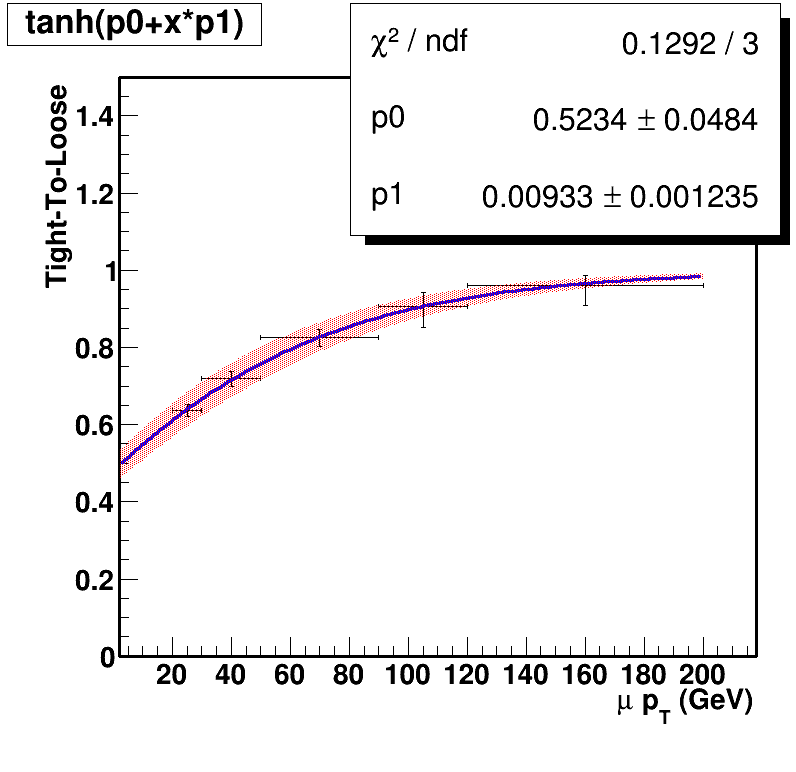
\includegraphics[width=0.3\textwidth]{plots/chapter7/Fake/FR/MMM2017.png}
    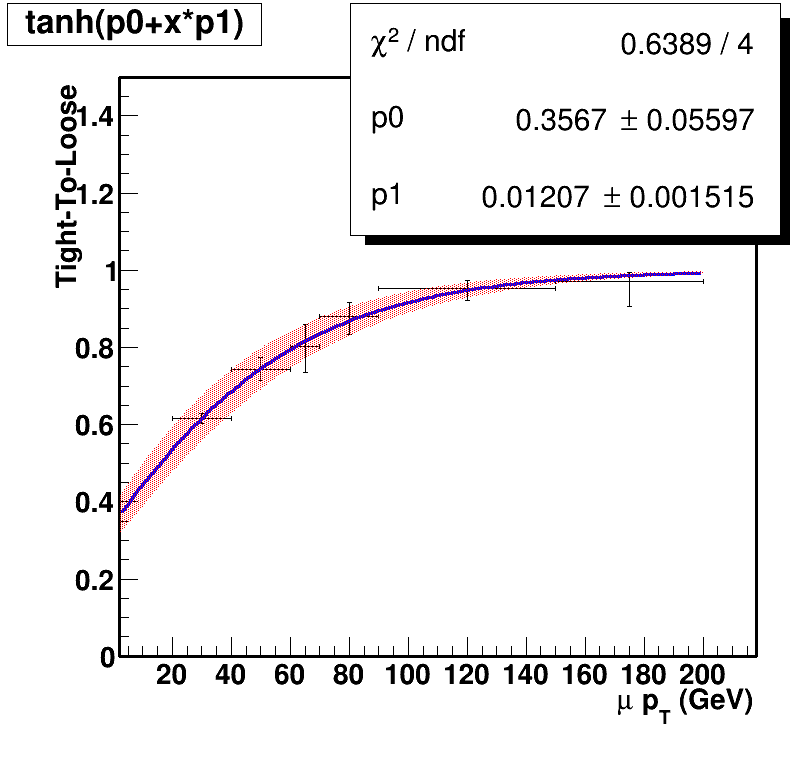
\includegraphics[width=0.3\textwidth]{plots/chapter7/Fake/FR/MMM2018.png}
  }
  \subfigure[]{
    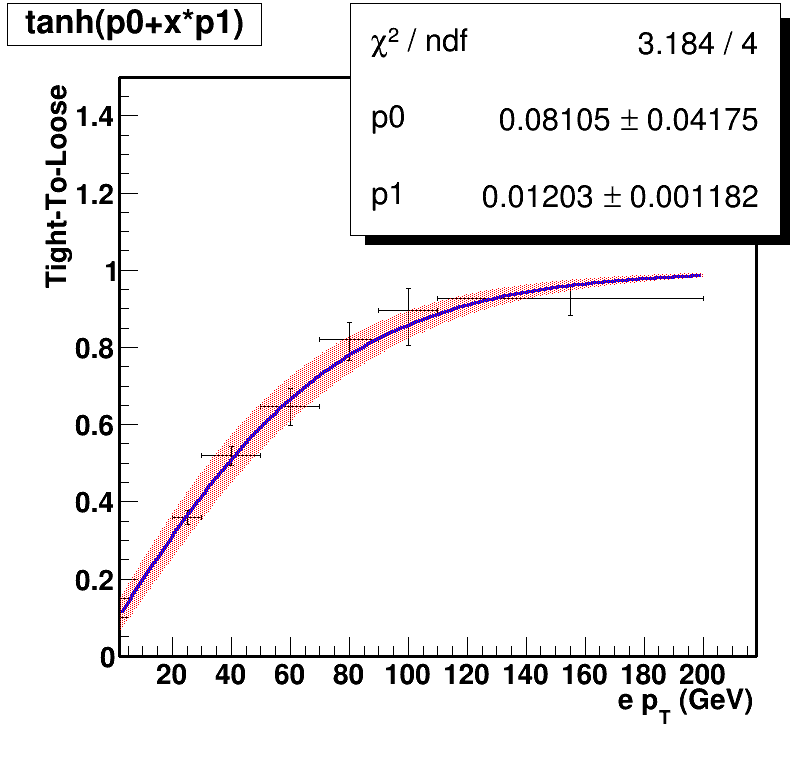
\includegraphics[width=0.3\textwidth]{plots/chapter7/Fake/FR/MME2016.png}
    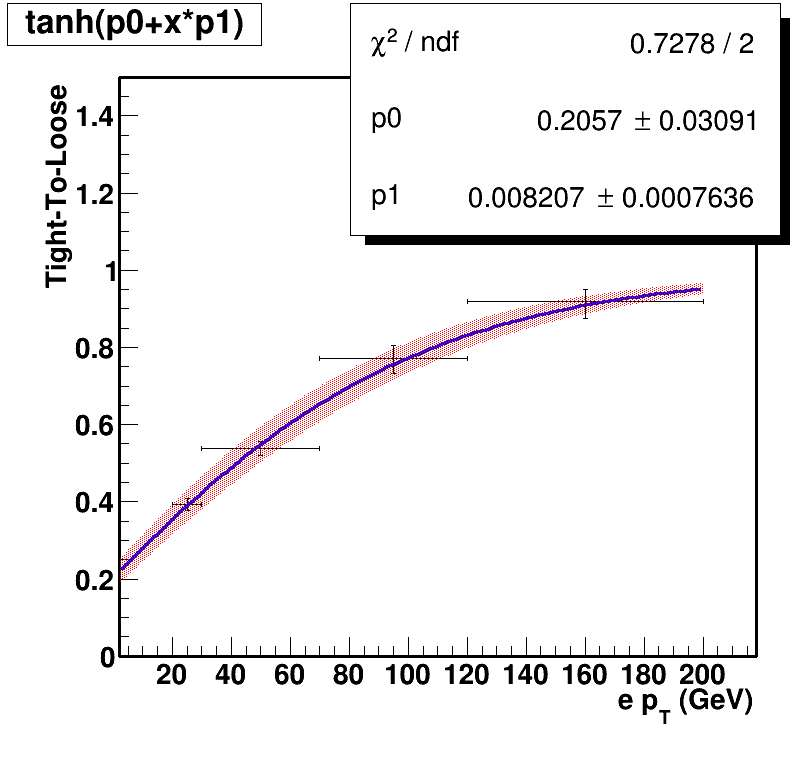
\includegraphics[width=0.3\textwidth]{plots/chapter7/Fake/FR/MME2017.png}
    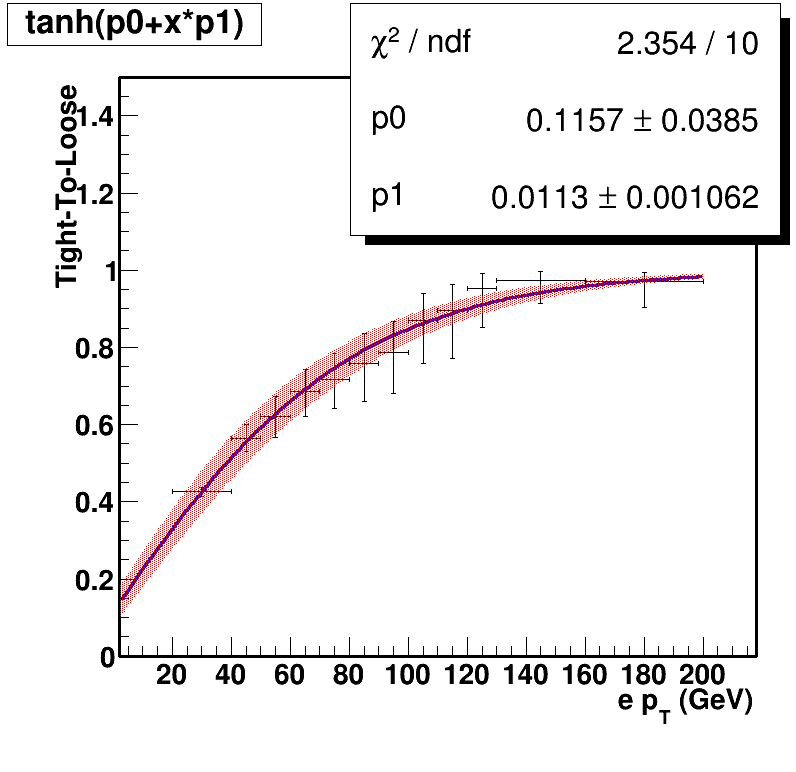
\includegraphics[width=0.3\textwidth]{plots/chapter7/Fake/FR/MME2018.png}
  }
  \caption{Fit performed to the \Pgm\, (a) and \Pe\, (b) misidentification rates as a function of their \pt\, for 2016 (Left), 2017 (Center), and 2018 (Right). The misidentification rates are labeled as ``tight-to-loose'' to clarify that they are calculated as a ratio of the number of events passing the tight isolation to the loose isolation. The hyperbolic tangent function is used for performing the fit.}
  \label{fig:fakerate_tauh}
\end{figure}

Each event in the control region defined using the collision data with the same selection as the signal region, but loosening the isolation requirements on one of the leptons is then weighted by a factor $f_i/(1-f_i)$ depending on the lepton \pt\, for electrons and muons or \pt, $\eta$ and decay mode for the \Pgt\, lepton candidates. Both background yields and shape distributions are thus estimated. Events with the possibility of double-counting due to two misidentified leptons are subtracted using a weight. For example, events with a misidentified \Pgm (\Pe) and a misidentified \tauh are subtracted in the \Hmuhad (\Hehad) channel using a weight, $f_\Pgt f_\ell/[(1-f_\Pgt)(1-f_\ell)]$, where $\ell = \Pgm$ or \Pe.

The estimation of the background is validated in events where the two leptons have the same electric charge. The misidentification rate $f_i$ is applied to events passing preselection and by inverting the lepton pair's charge requirement. The same-sign selection enhances the misidentified lepton background. The background estimation is also validated in a \PW\, boson enriched control sample. This control region is obtained by applying the signal-like requirement and $\mt(\ell, \ptvecmiss) > 60\GeV$ ($\ell=\Pe$ or \Pgm) and $\mt(\tauh, \ptvecmiss) > 80\GeV$. The same strategy is applied in the \Hehad channel, which results in a similar agreement. Figures ~\ref{fig:fake_control} and ~\ref{fig:fake_control_BDT} show the comparison of data with background estimates in the same-sign and \PW\, boson enriched control regions for the \Hmuhad and \Hehad channels.

\begin{figure}[htbp!]
  \centering
  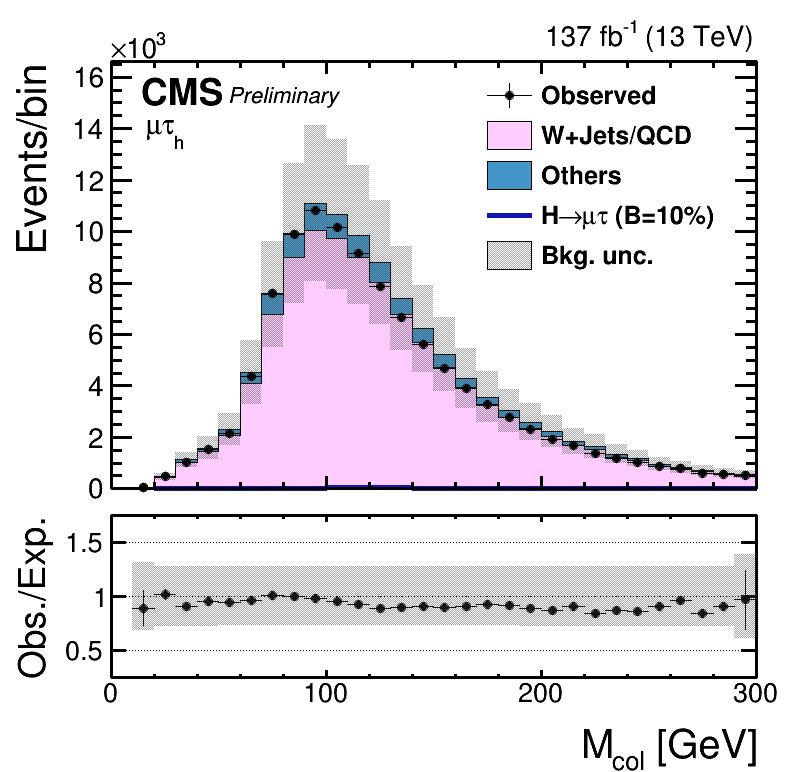
\includegraphics[width=0.45\textwidth]{plots/chapter7/Fake/mutau/SS.png}
  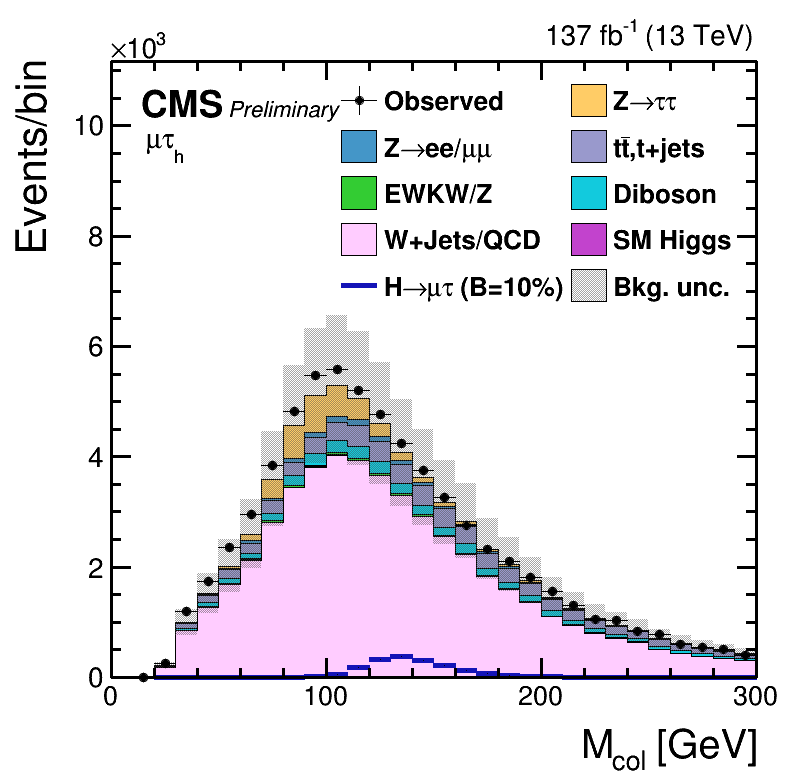
\includegraphics[width=0.45\textwidth]{plots/chapter7/Fake/mutau/WOS.png}
  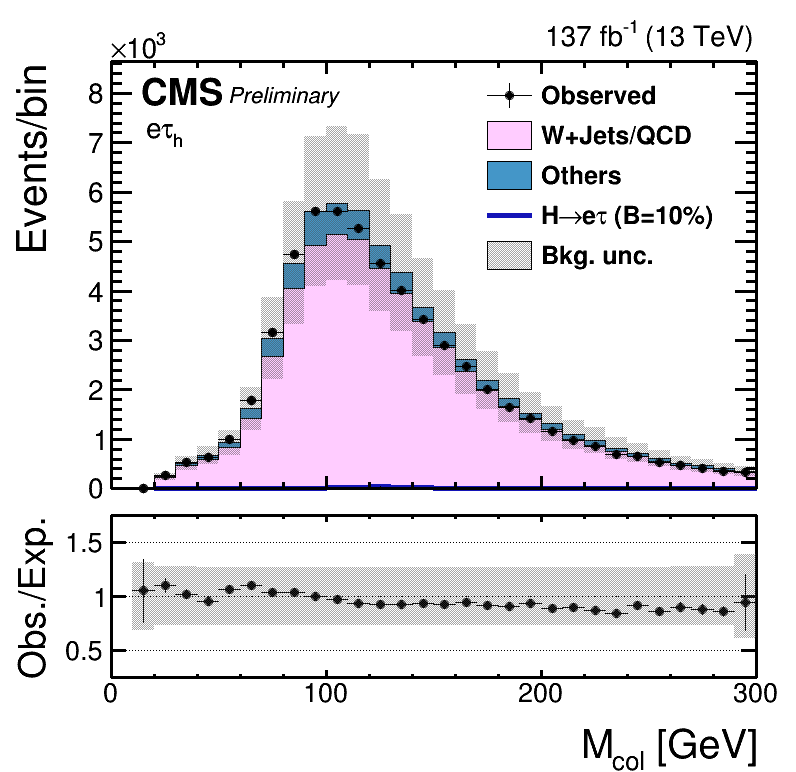
\includegraphics[width=0.45\textwidth]{plots/chapter7/Fake/etau/SS.png}
  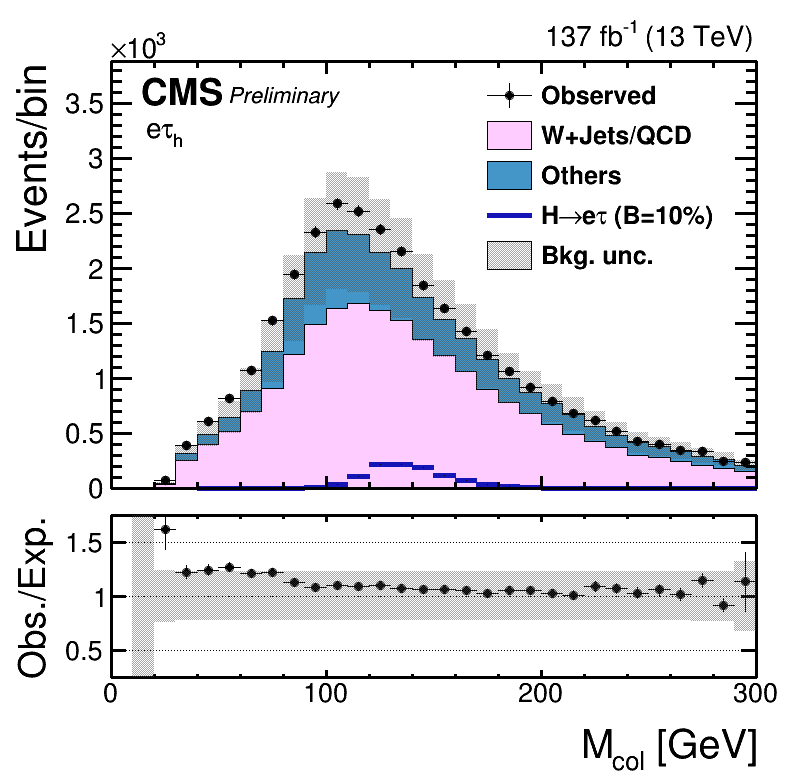
\includegraphics[width=0.45\textwidth]{plots/chapter7/Fake/etau/WOS.png}
  \caption{Distributions of \mcol discriminator in the same-sign (Left) and \PW\, boson enriched (Right) control regions for the \Hmuhad (top) and \Hehad (bottom) channels.}
  \label{fig:fake_control}
\end{figure}

\begin{figure}[htbp!]
  \centering
  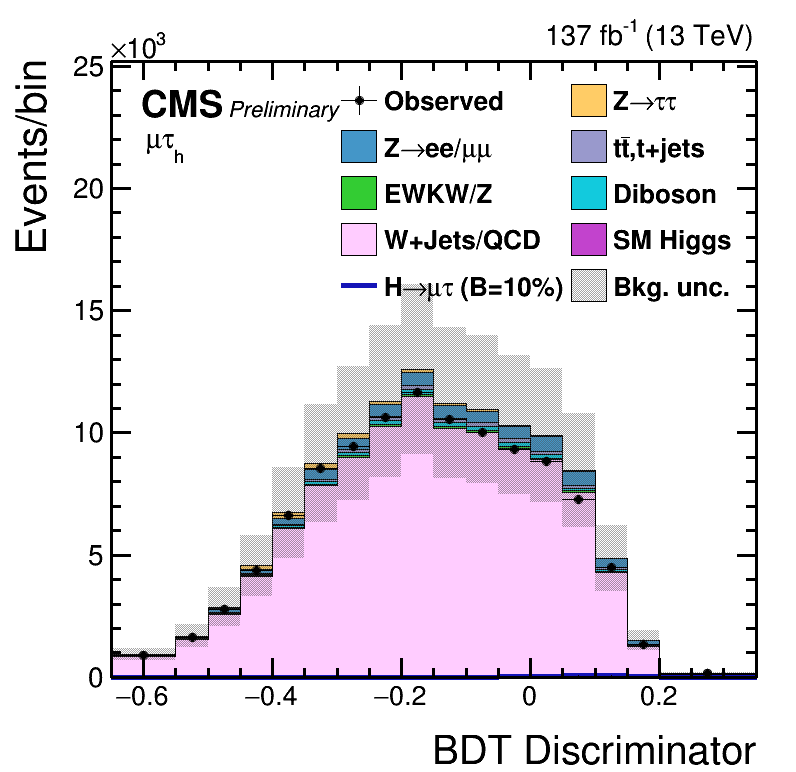
\includegraphics[width=0.45\textwidth]{plots/chapter7/Fake/mutau/SSBDT.png}
  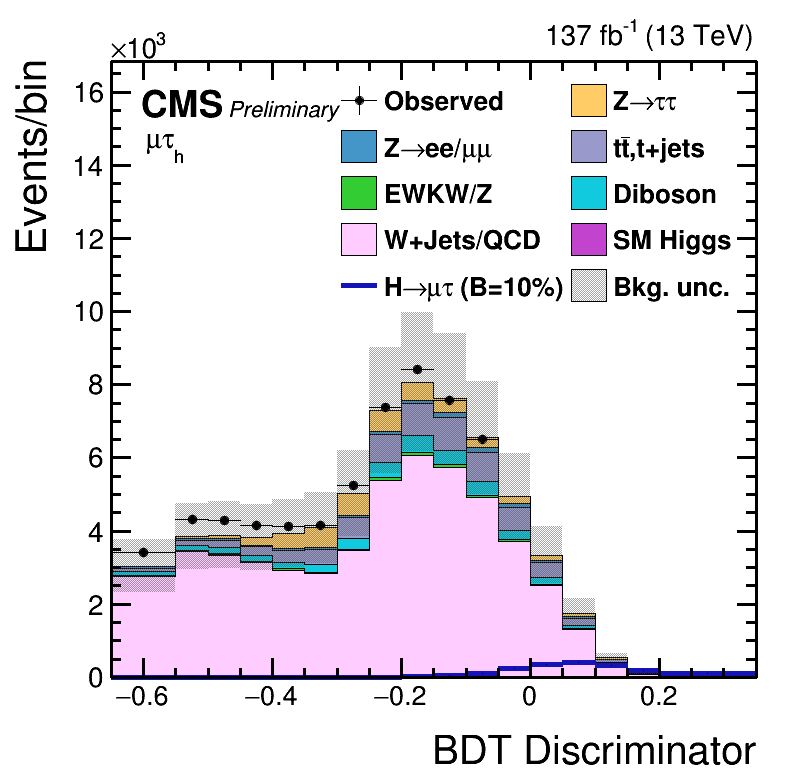
\includegraphics[width=0.45\textwidth]{plots/chapter7/Fake/mutau/WOSBDT.png}
  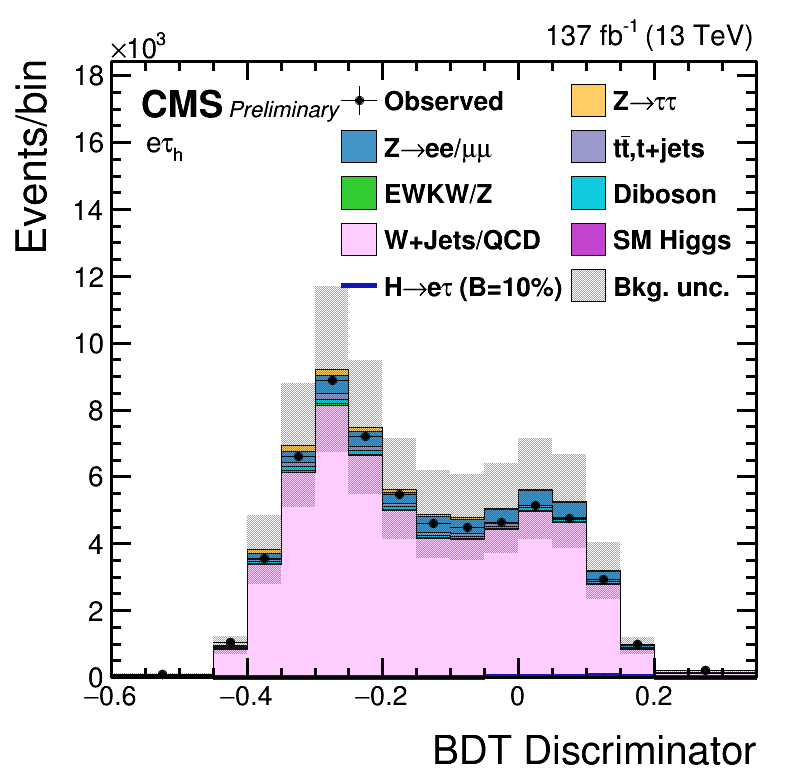
\includegraphics[width=0.45\textwidth]{plots/chapter7/Fake/etau/SSBDT.png}
  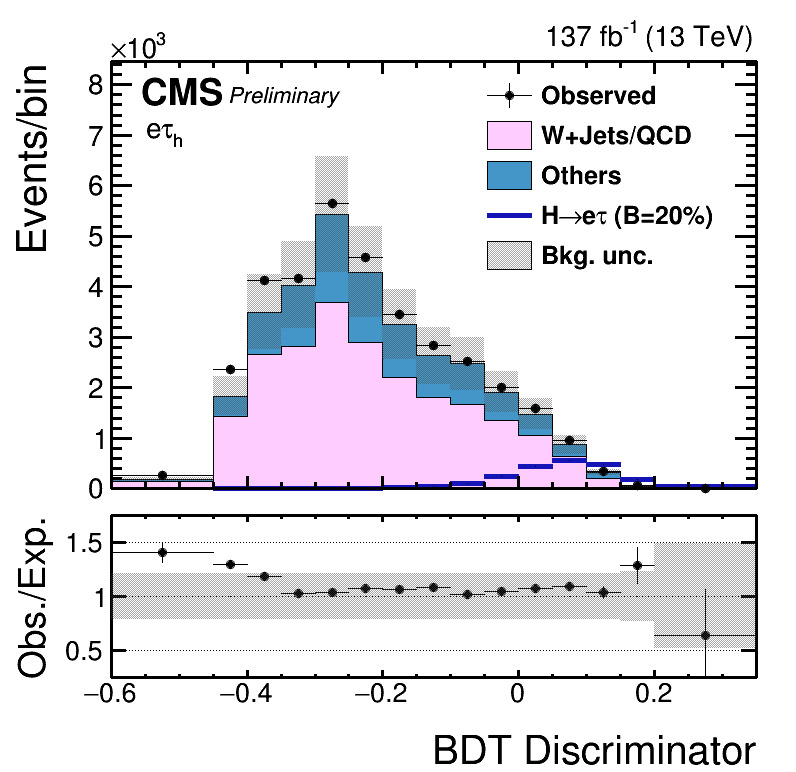
\includegraphics[width=0.45\textwidth]{plots/chapter7/Fake/etau/WOSBDT.png}
  \caption{Distributions of BDT discriminator in the same-sign (Left) and \PW\, boson enriched (Right) control regions for the \Hmuhad (top) and \Hehad (bottom) channels.}
  \label{fig:fake_control_BDT}
\end{figure}

\subsection{Semi data-driven approach}
In the \Hemu and \Hmue channels, QCD multijet background is estimated from data using events with an electron and a muon with the same electric charge. These events are selected by applying the preselection except for requiring both the leptons to have the same electric charge, and we call this the same sign (SS) control region. Contributions from other processes are estimated from simulation and subtracted from data in this SS control region. Extrapolation factors from the SS control region to the opposite sign (OS) signal region are measured in data as a function of the jet multiplicity and the $\Delta R$ separation between the electron and the muon. QCD OS/SS extrapolation factors that are measured can be seen in Figure ~\ref{fig:osss}.

\begin{figure}[htbp]
  \centering
  \subfigure[]{
    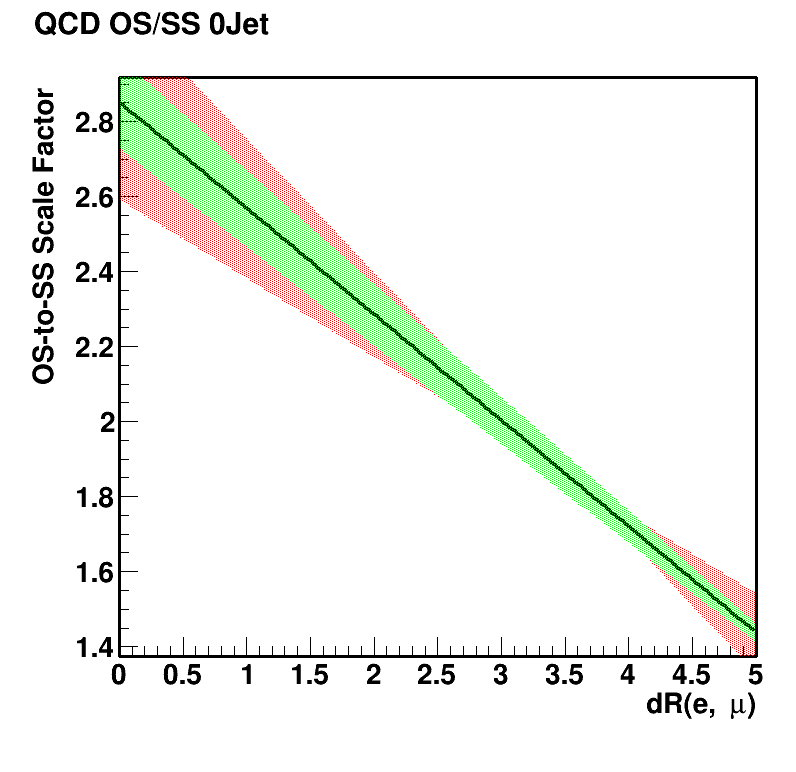
\includegraphics[width=0.3\textwidth]{plots/chapter7/QCD/2016/0Jet.png}
    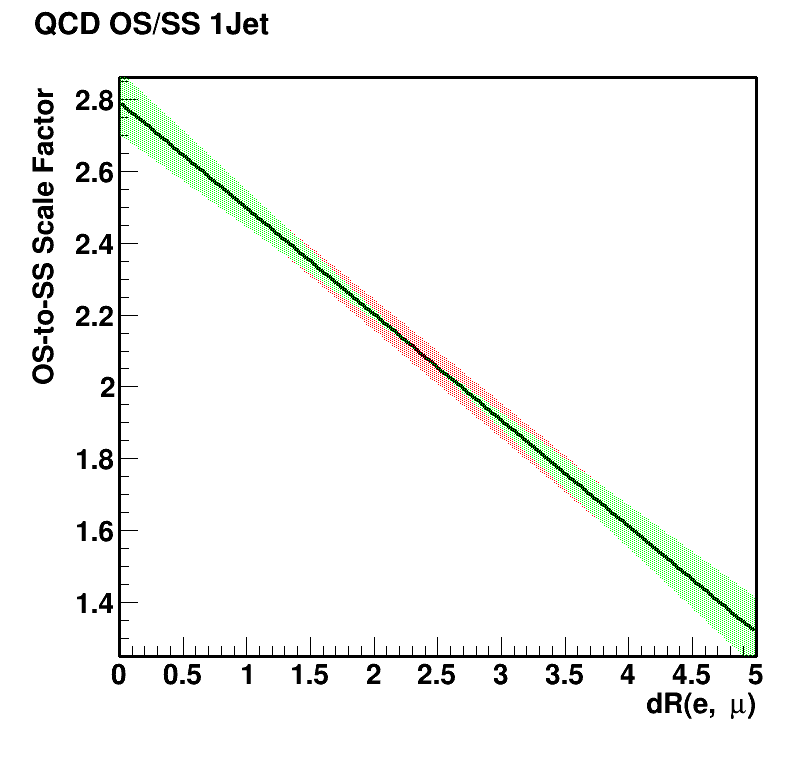
\includegraphics[width=0.3\textwidth]{plots/chapter7/QCD/2016/1Jet.png}
    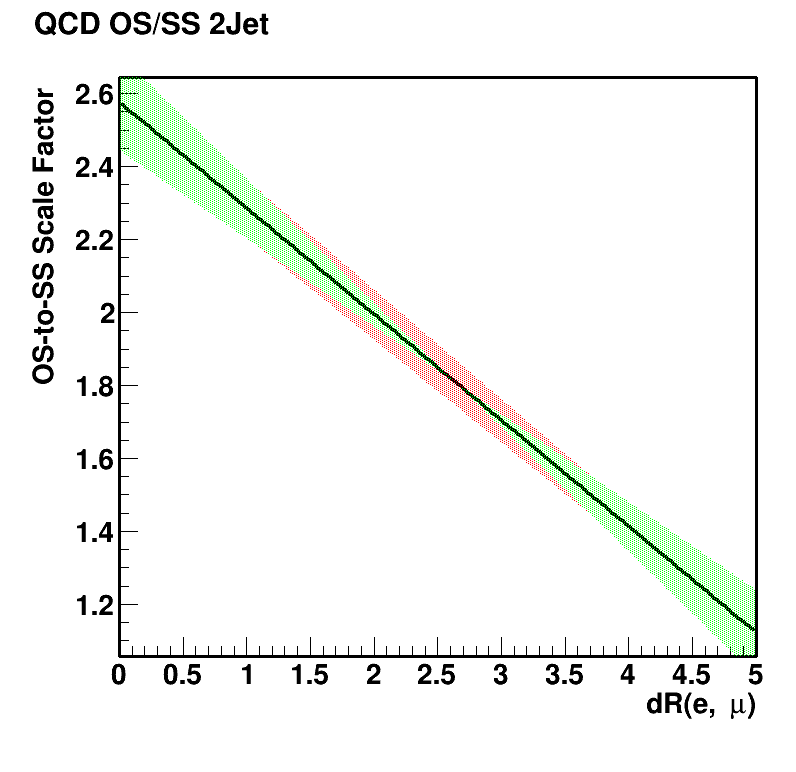
\includegraphics[width=0.3\textwidth]{plots/chapter7/QCD/2016/2Jet.png}
  }
  \subfigure[]{
    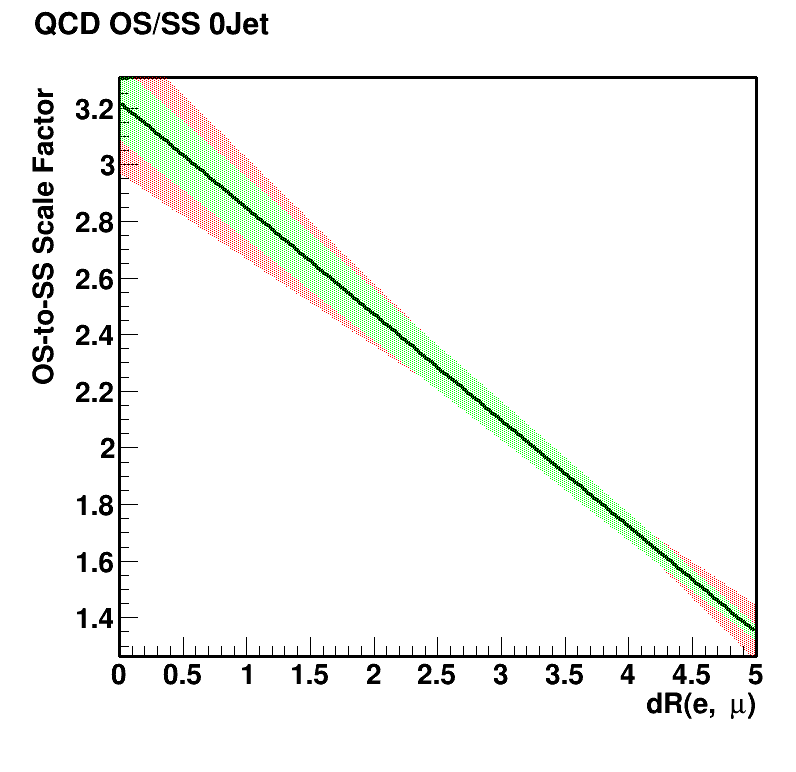
\includegraphics[width=0.3\textwidth]{plots/chapter7/QCD/2017/0Jet.png}
    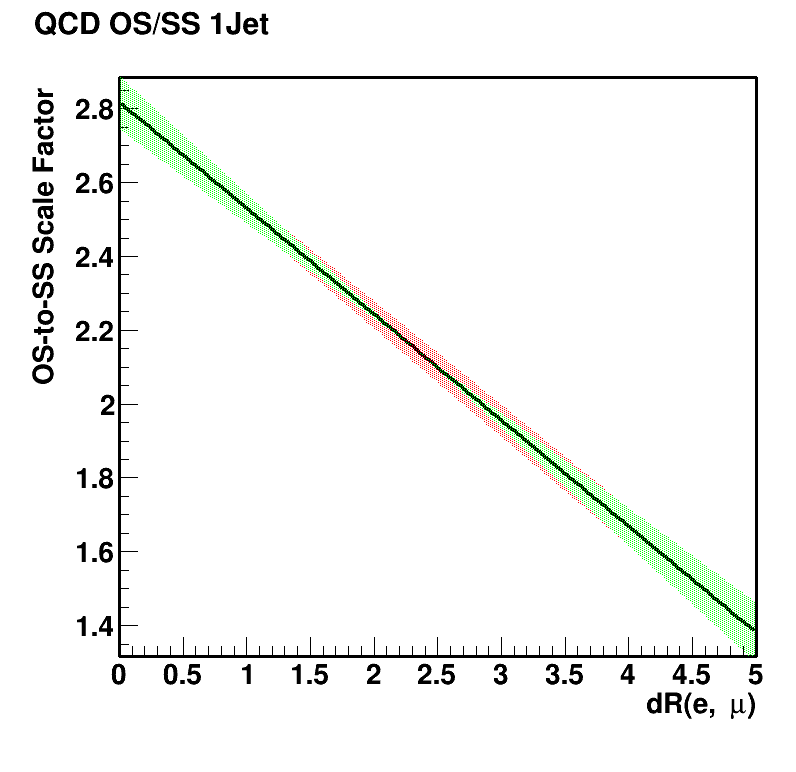
\includegraphics[width=0.3\textwidth]{plots/chapter7/QCD/2017/1Jet.png}
    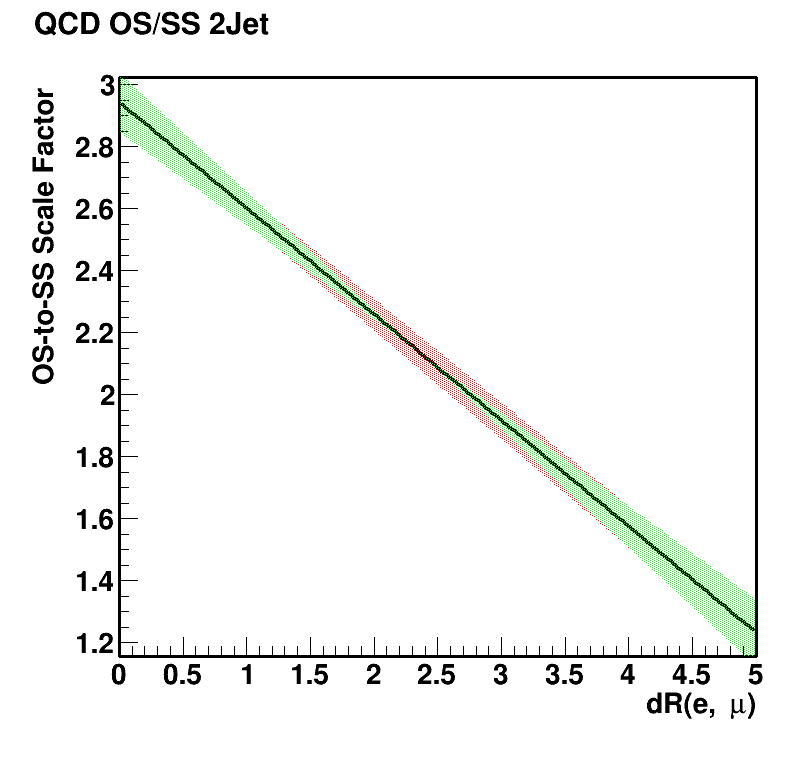
\includegraphics[width=0.3\textwidth]{plots/chapter7/QCD/2017/2Jet.png}
  }
  \subfigure[]{
    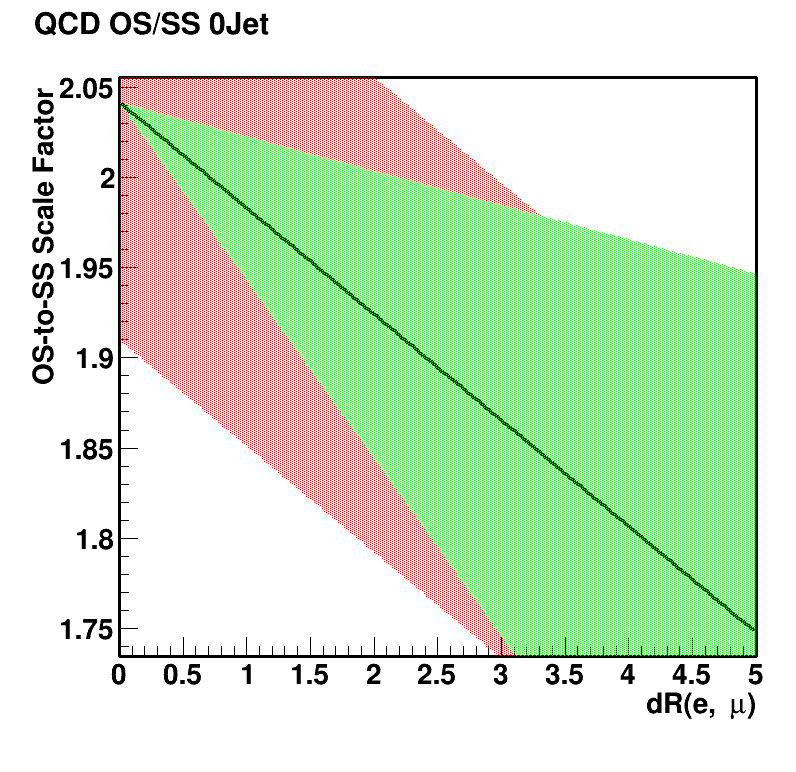
\includegraphics[width=0.3\textwidth]{plots/chapter7/QCD/2018/0Jet.png}
    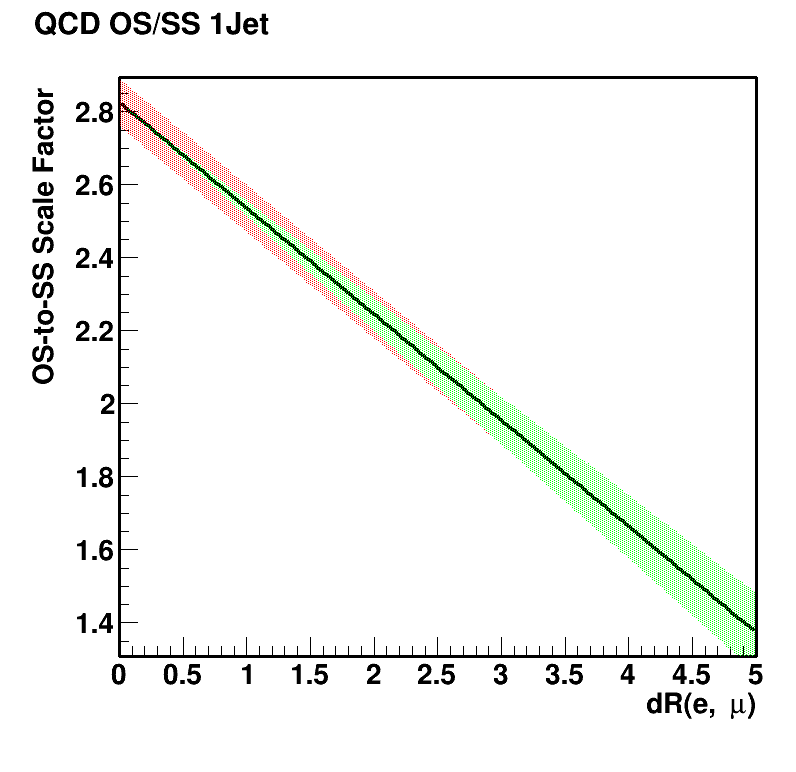
\includegraphics[width=0.3\textwidth]{plots/chapter7/QCD/2018/1Jet.png}
    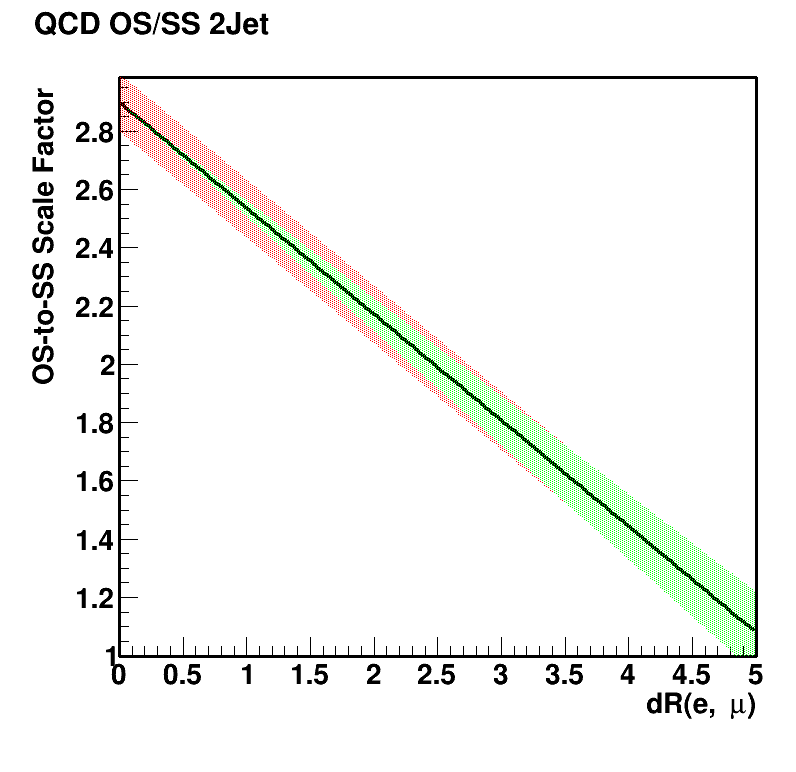
\includegraphics[width=0.3\textwidth]{plots/chapter7/QCD/2018/2Jet.png}
  }
  \caption{QCD OS/SS extrapolation factors in events with 0 Jets (Left), 1 Jet (Center), and 2 Jets (Right) for 2016 (a), 2017 (b), 2018 (c). The line is the best fit, and the shaded region corresponds to the shape uncertainties.}
  \label{fig:osss}
\end{figure}

The OS/SS extrapolation factor is estimated using events with an anti-isolated muon and an isolated electron. The contribution from $b\bar{b}$ events to the QCD multijet background gives rise to the $\Delta R$ dependency and is parameterized with a linear function. The OS/SS extrapolation factor is higher for events with low $\Delta R $ separation between the electron and the muon, decreasing as the $\Delta R $ separation increases. The OS/SS extrapolation factor also depends on the electron and muon \pt. This \pt\, dependence comes from the leptons arising from the semi-leptonic c quark decay. These leptons tend to be softer in \pt\, and less isolated resulting in a reduction in the number of such events passing the \pt\, and isolation requirements. Corrections of the QCD OS/SS extrapolation factors dependent on lepton \pt\, along with the correction to account for the mismodeling introduced by anti-isolating the muon to measure them can be seen in Figure ~\ref{fig:osss_corr}.

\begin{figure}[htbp]
  \centering
  \subfigure[]{
    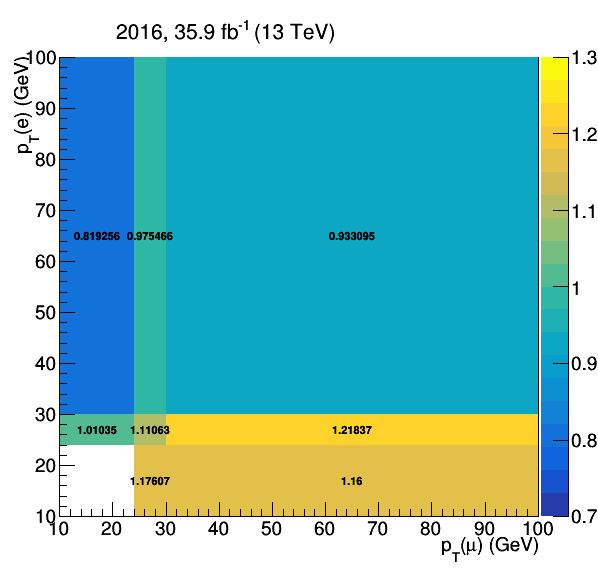
\includegraphics[width=0.3\textwidth]{plots/chapter7/QCD/2016/pt.png}
    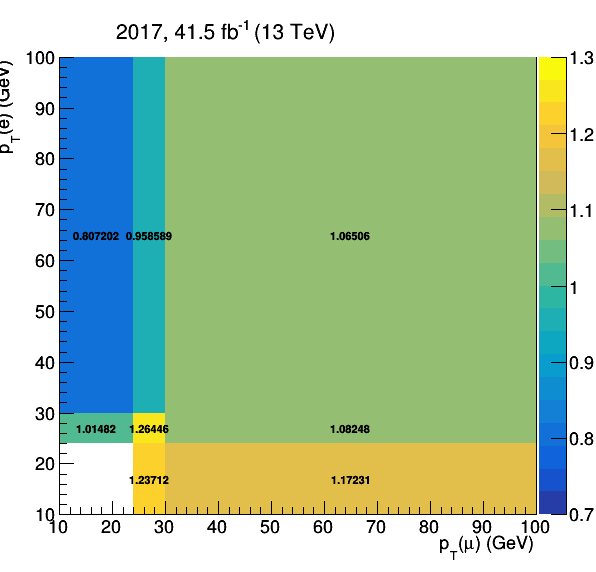
\includegraphics[width=0.3\textwidth]{plots/chapter7/QCD/2017/pt.png}
    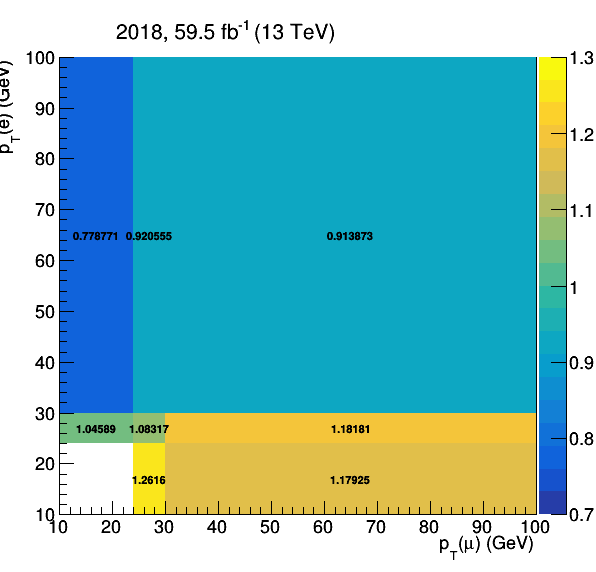
\includegraphics[width=0.3\textwidth]{plots/chapter7/QCD/2018/pt.png}
  }
  \subfigure[]{
    \includegraphics[width=0.3\textwidth]{plots/chapter7/QCD/2016/iso.png}
    \includegraphics[width=0.3\textwidth]{plots/chapter7/QCD/2017/iso.png}
    \includegraphics[width=0.3\textwidth]{plots/chapter7/QCD/2018/iso.png}
  }
  \caption{(a) Corrections of the QCD OS/SS extrapolation factors determined in the region with an anti-isolated muon as a function of the \pt\, of the electron and the muon, using data collected in 2016, 2017, and 2018. (b) Correction of the QCD OS/SS extrapolation factors to account for the mismodeling introduced by anti-isolating the muon to measure the SFs, using data collected in 2016, 2017, and 2018.}
  \label{fig:osss_corr}
\end{figure}

As the OS/SS extrapolation factor is measured in a control region where the muon is anti-isolated, an additional correction is applied to cover for a potential mismodeling. This correction is calculated by measuring the OS/SS extrapolation factors in two different control regions. The first control region has events where the muon is isolated, and the electron is anti-isolated. The second control region has events where both the electron and the muon are anti-isolated. The ratio of the extrapolation factors measured in these two control regions is taken as the correction for accounting the potential mismodeling induced by anti-isolating the muon. Figure ~\ref{fig:qcd_control} shows the comparison of data with background estimates in the muon anti-isolated control regions for the \Hmue channel.

\begin{figure}[htbp!]
  \centering
  \includegraphics[width=0.45\textwidth]{plots/chapter7/Fake/mue/QCD.png}
  \caption{Distribution of \mcol discriminator in the muon anti-isolated control regions for the \Hmue channel.}
  \label{fig:qcd_control}
\end{figure}

\section{MC Simulation}
All the other backgrounds are estimated using MC simulation. In the leptonic channels, the \ttbar process has a dominant contribution, and this background is validated in a dedicated control region defined by requiring the presence of at least one b jet tagged by the DeepCSV algorithm in the event. Figure ~\ref{fig:tt_control} shows the background validation in this control region for the \Hmue and \Hemu channels.

The standard model, Higgs boson production, forms a small but non-negligible background. The contributions come mainly from \Htt and \HWW decays. The contribution from \HWW peaks at lower values than the signal in the distribution of the BDT discriminator due to the presence of additional neutrinos in the decay. The background is estimated from simulations using selection based on the BDT discriminator and kinematic variables, as described in Chapter ~\ref{evt_sel}.

\begin{figure}[htbp!]
  \centering
  \includegraphics[width=0.45\textwidth]{plots/chapter7/Fake/mue/TT.png}
  \includegraphics[width=0.45\textwidth]{plots/chapter7/Fake/emu/TT.png}
  \includegraphics[width=0.45\textwidth]{plots/chapter7/Fake/mue/TTBDT.png}
  \includegraphics[width=0.45\textwidth]{plots/chapter7/Fake/emu/TTBDT.png}
  \caption{Distributions of \mcol (BDT) discriminator in \ttbar enriched control region for \Hmue and \Hemu channel.}
  \label{fig:tt_control}
\end{figure}

%
% % % uncomment the following lines,
% % if using chapter-wise bibliography
% %
% % \bibliographystyle{ndnatbib}
% % \bibliography{example}
